\documentclass[a4paper,12pt,titlepage]{article}

\usepackage[pdftex]{graphicx}
\usepackage[headheight=15pt]{geometry}

\usepackage{fancyhdr}
\pagestyle{fancy}
\lhead{OpenStreetMap}
\chead{}
\rhead{Practical Guideline}

\usepackage[english]{babel}									
\usepackage[utf8]{inputenc}	

\usepackage{array}
\usepackage{colortbl}

\usepackage[section]{placeins}
\usepackage{float}

%PDF hyperlinks
\usepackage[colorlinks=true,linkcolor=orange,bookmarksopen=true,bookmarksnumbered=false,pdfstartpage=2]{hyperref}

\usepackage{color}
\definecolor{orange}{rgb}{1,.5,0}

\title{Guideline for OSM contribution and use}
\author{Michael Wagner}
\date{\today}

\clubpenalty=4500	
\widowpenalty=10000
\linespread{1.3}

%%-------------------------Document begins--------------------------------------------
\begin{document}
\maketitle

\tableofcontents
\listoffigures
\newpage

\section{Introduction}

OpenStreetMap (OSM) is a great approach/tool/technology to share spatial data among organisations (and of course with the public). One of the main advantages of OSM is that required hardware, software and network infrastructure are already provided and can be used at no cost. The only thing organisations need to contribute to OSM and use it is an Internet connection.
This guideline shows through an example how data on buildings can be prepared for upload to OSM and later on be used by the organisations within their own GIS software. The \textit{building} layer is one of the most useful layers in the Seychelles since many organisations maintain information that is directly or indirectly related to buildings. Using OSM can help these organisations to eliminate duplication and fragmentation of building relating data.

\section{Creating building data based on a GPS survey}

One way to capture missing building footprints is through the use of a (hand-held) GPS device. The result is usually a GPX file containing the coordinates of the building corners as waypoints. Such GPX file can then be loaded into JOSM. From the \textit{File} menu of JOSM select \textit{Open} and select your GPX file. The GPX file will be loaded into JOSM as a separate layer (Figure \ref{fig:load_gpx}).

\begin{figure}[H]
\centering
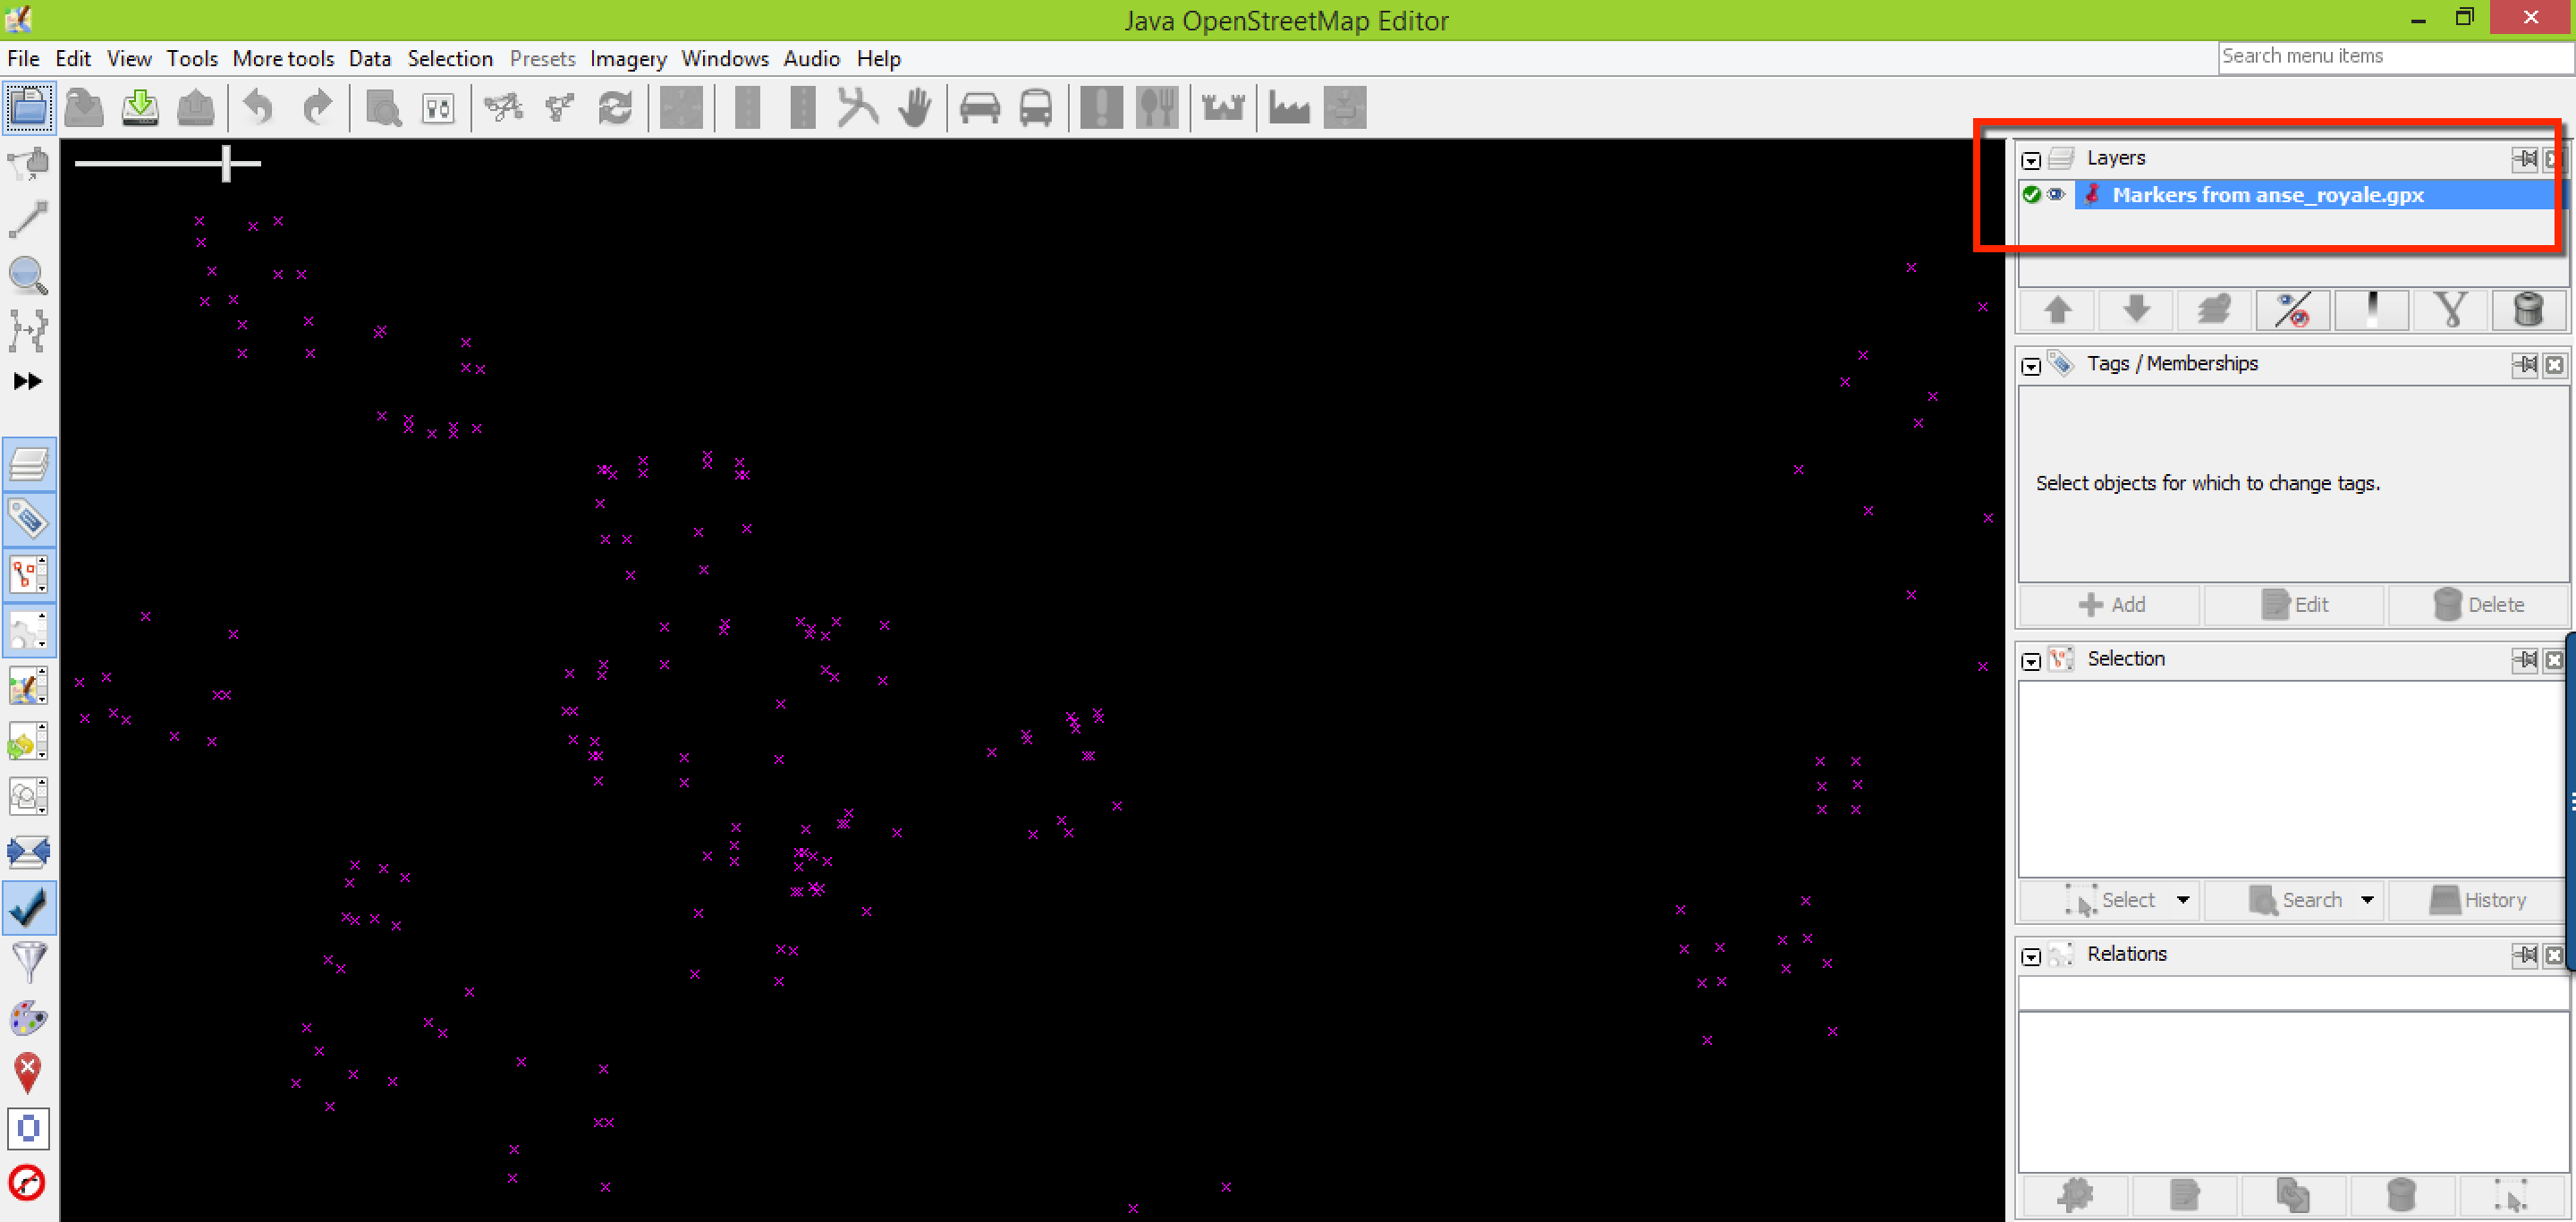
\includegraphics[width=12cm]{Images/load_gpx_file.png}
\caption{GPX file loaded into JOSM}\label{fig:load_gpx}
\end{figure}

Click the \textit{Download map data from the OSM server} button to download OSM data for the area you imported the GPX file for. JOSM recognizes the extent of your GPX data and will automatically offer to download data for that area only (Figure \ref{fig:load_gpx}). Make sure to toggle the checkbox \textit{Download as new layer}. To see existing OSM data next to your own data will facilitate your work and avoid duplication of data.  

\begin{figure}[H]
	\centering
	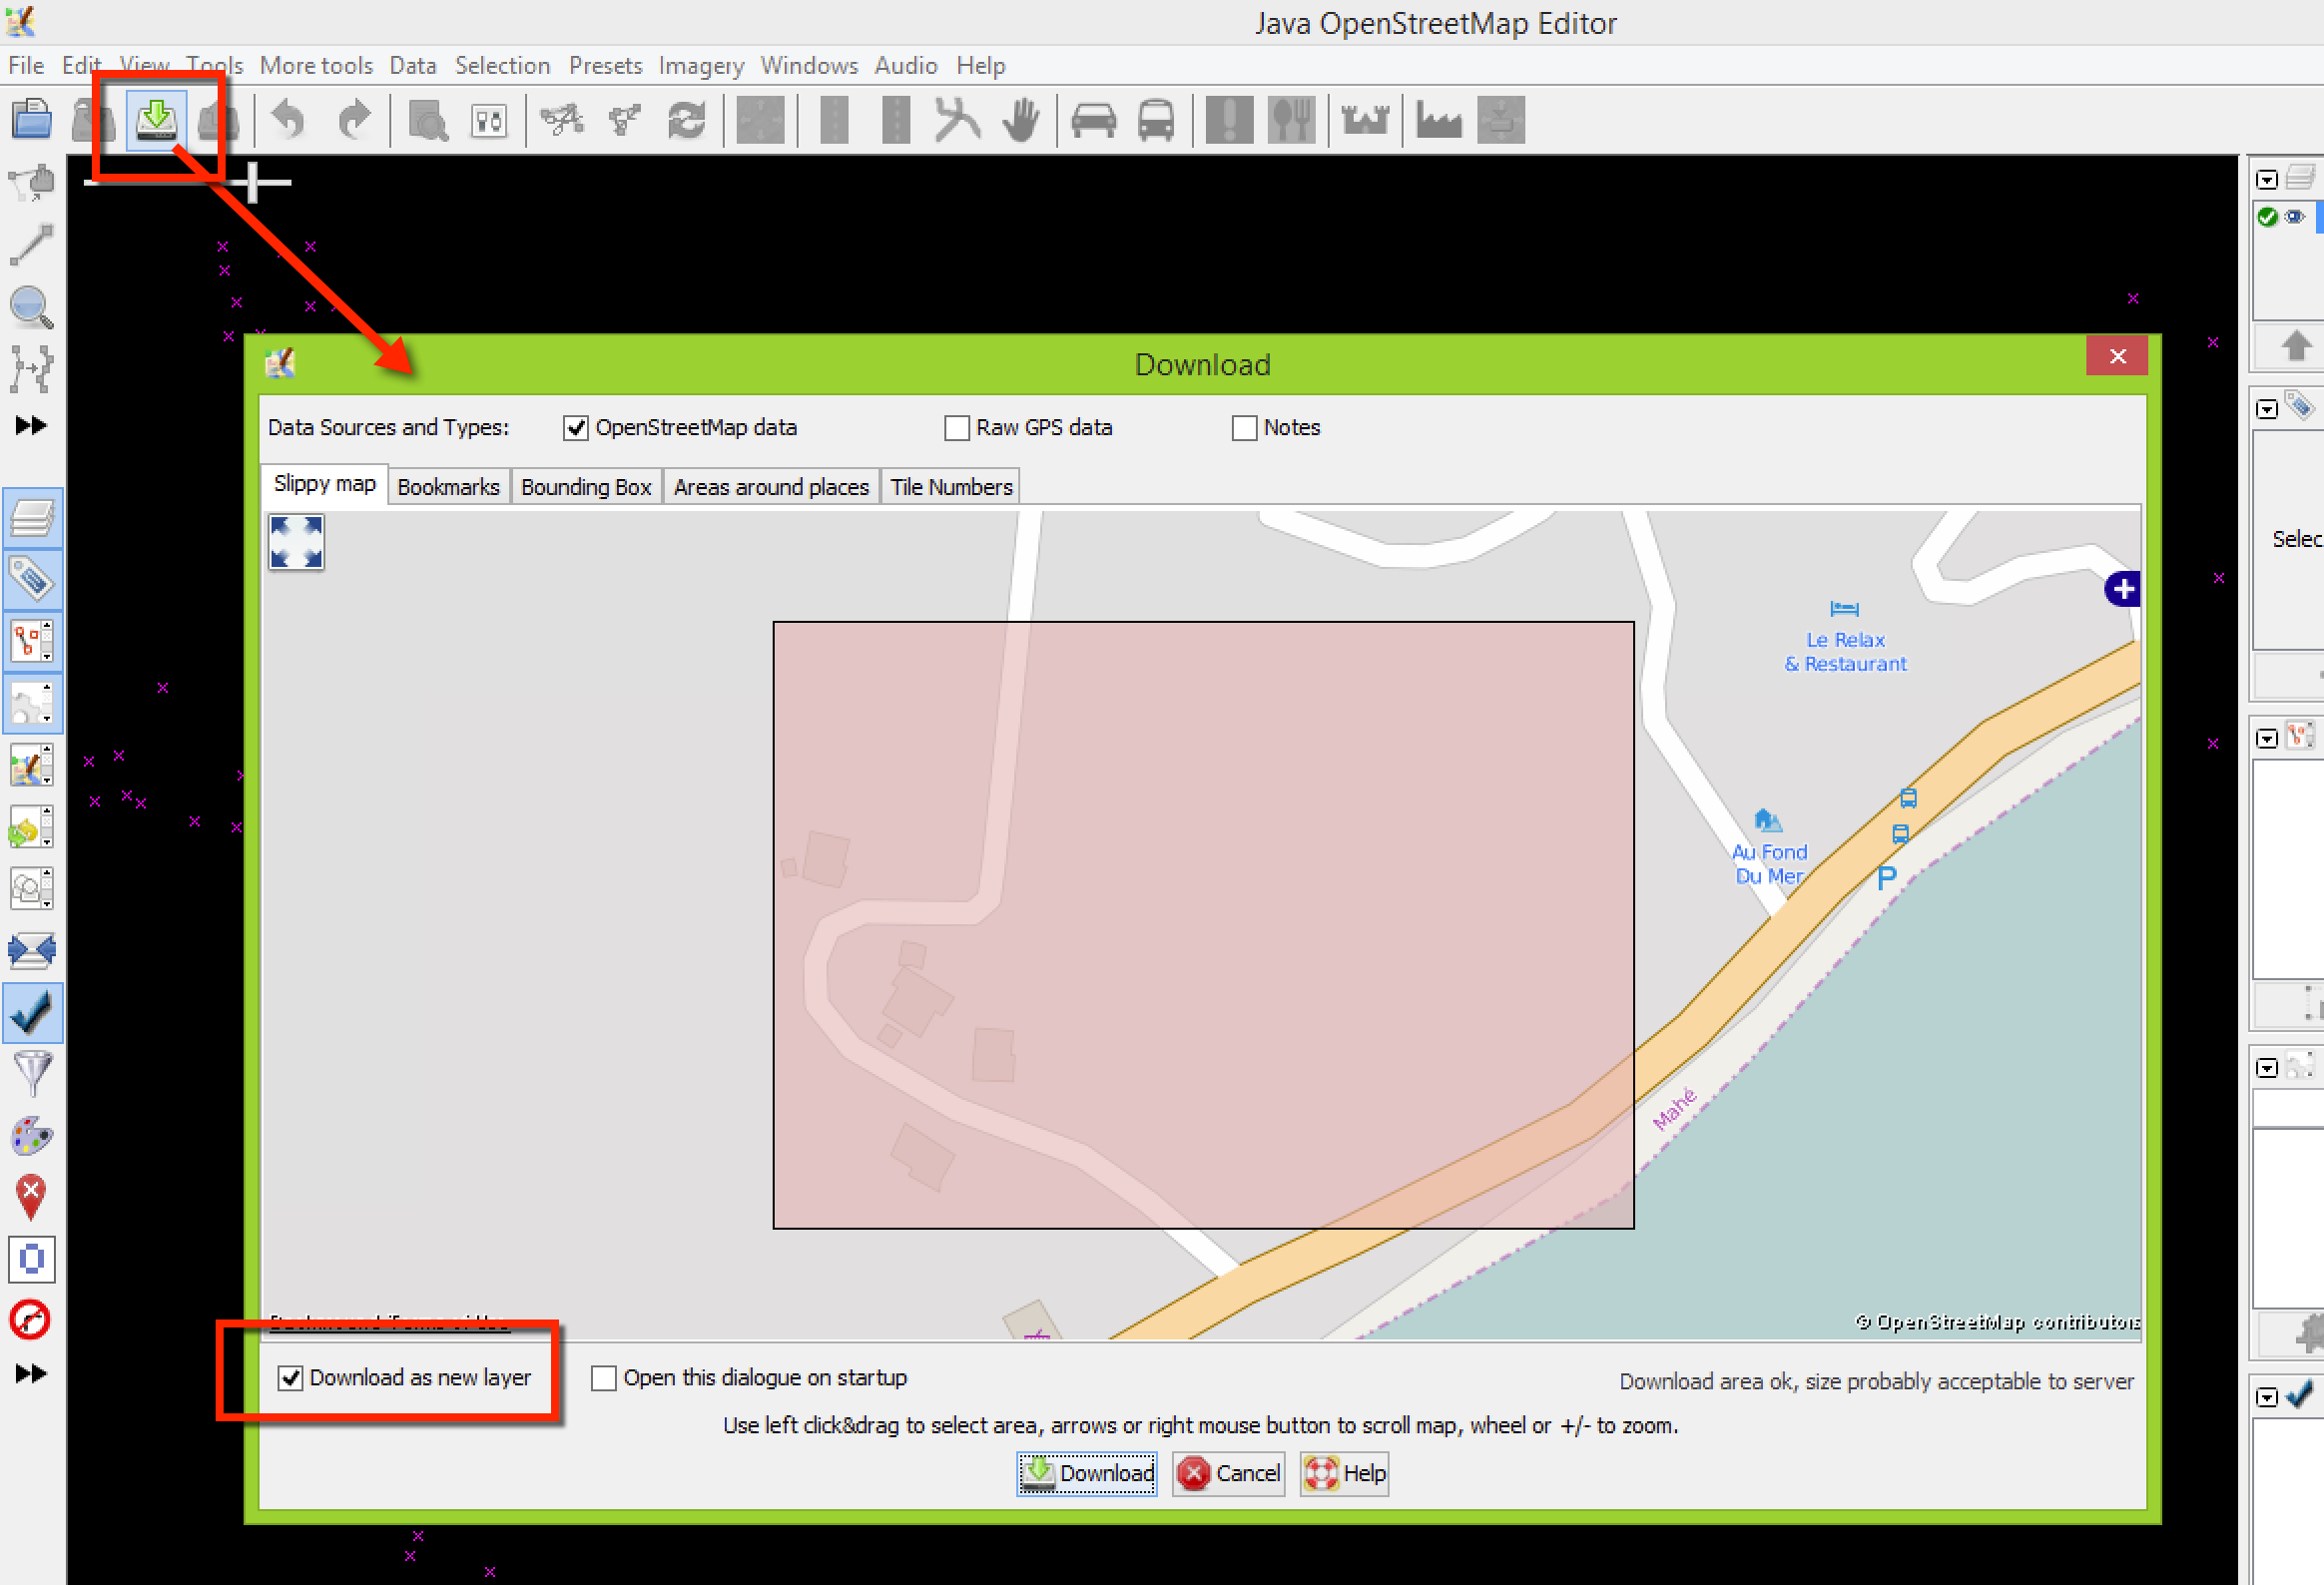
\includegraphics[width=12cm]{Images/load_gpx_file_2.png}
	\caption{Download data from OSM server}\label{fig:load_gpx_2}
\end{figure}

Depending on the area of your GPX data there might not be much OSM data available yet. Figure (\ref*{fig:load_gpx_3}) shows a few building footprints and some roads.

\begin{figure}[H]
	\centering
	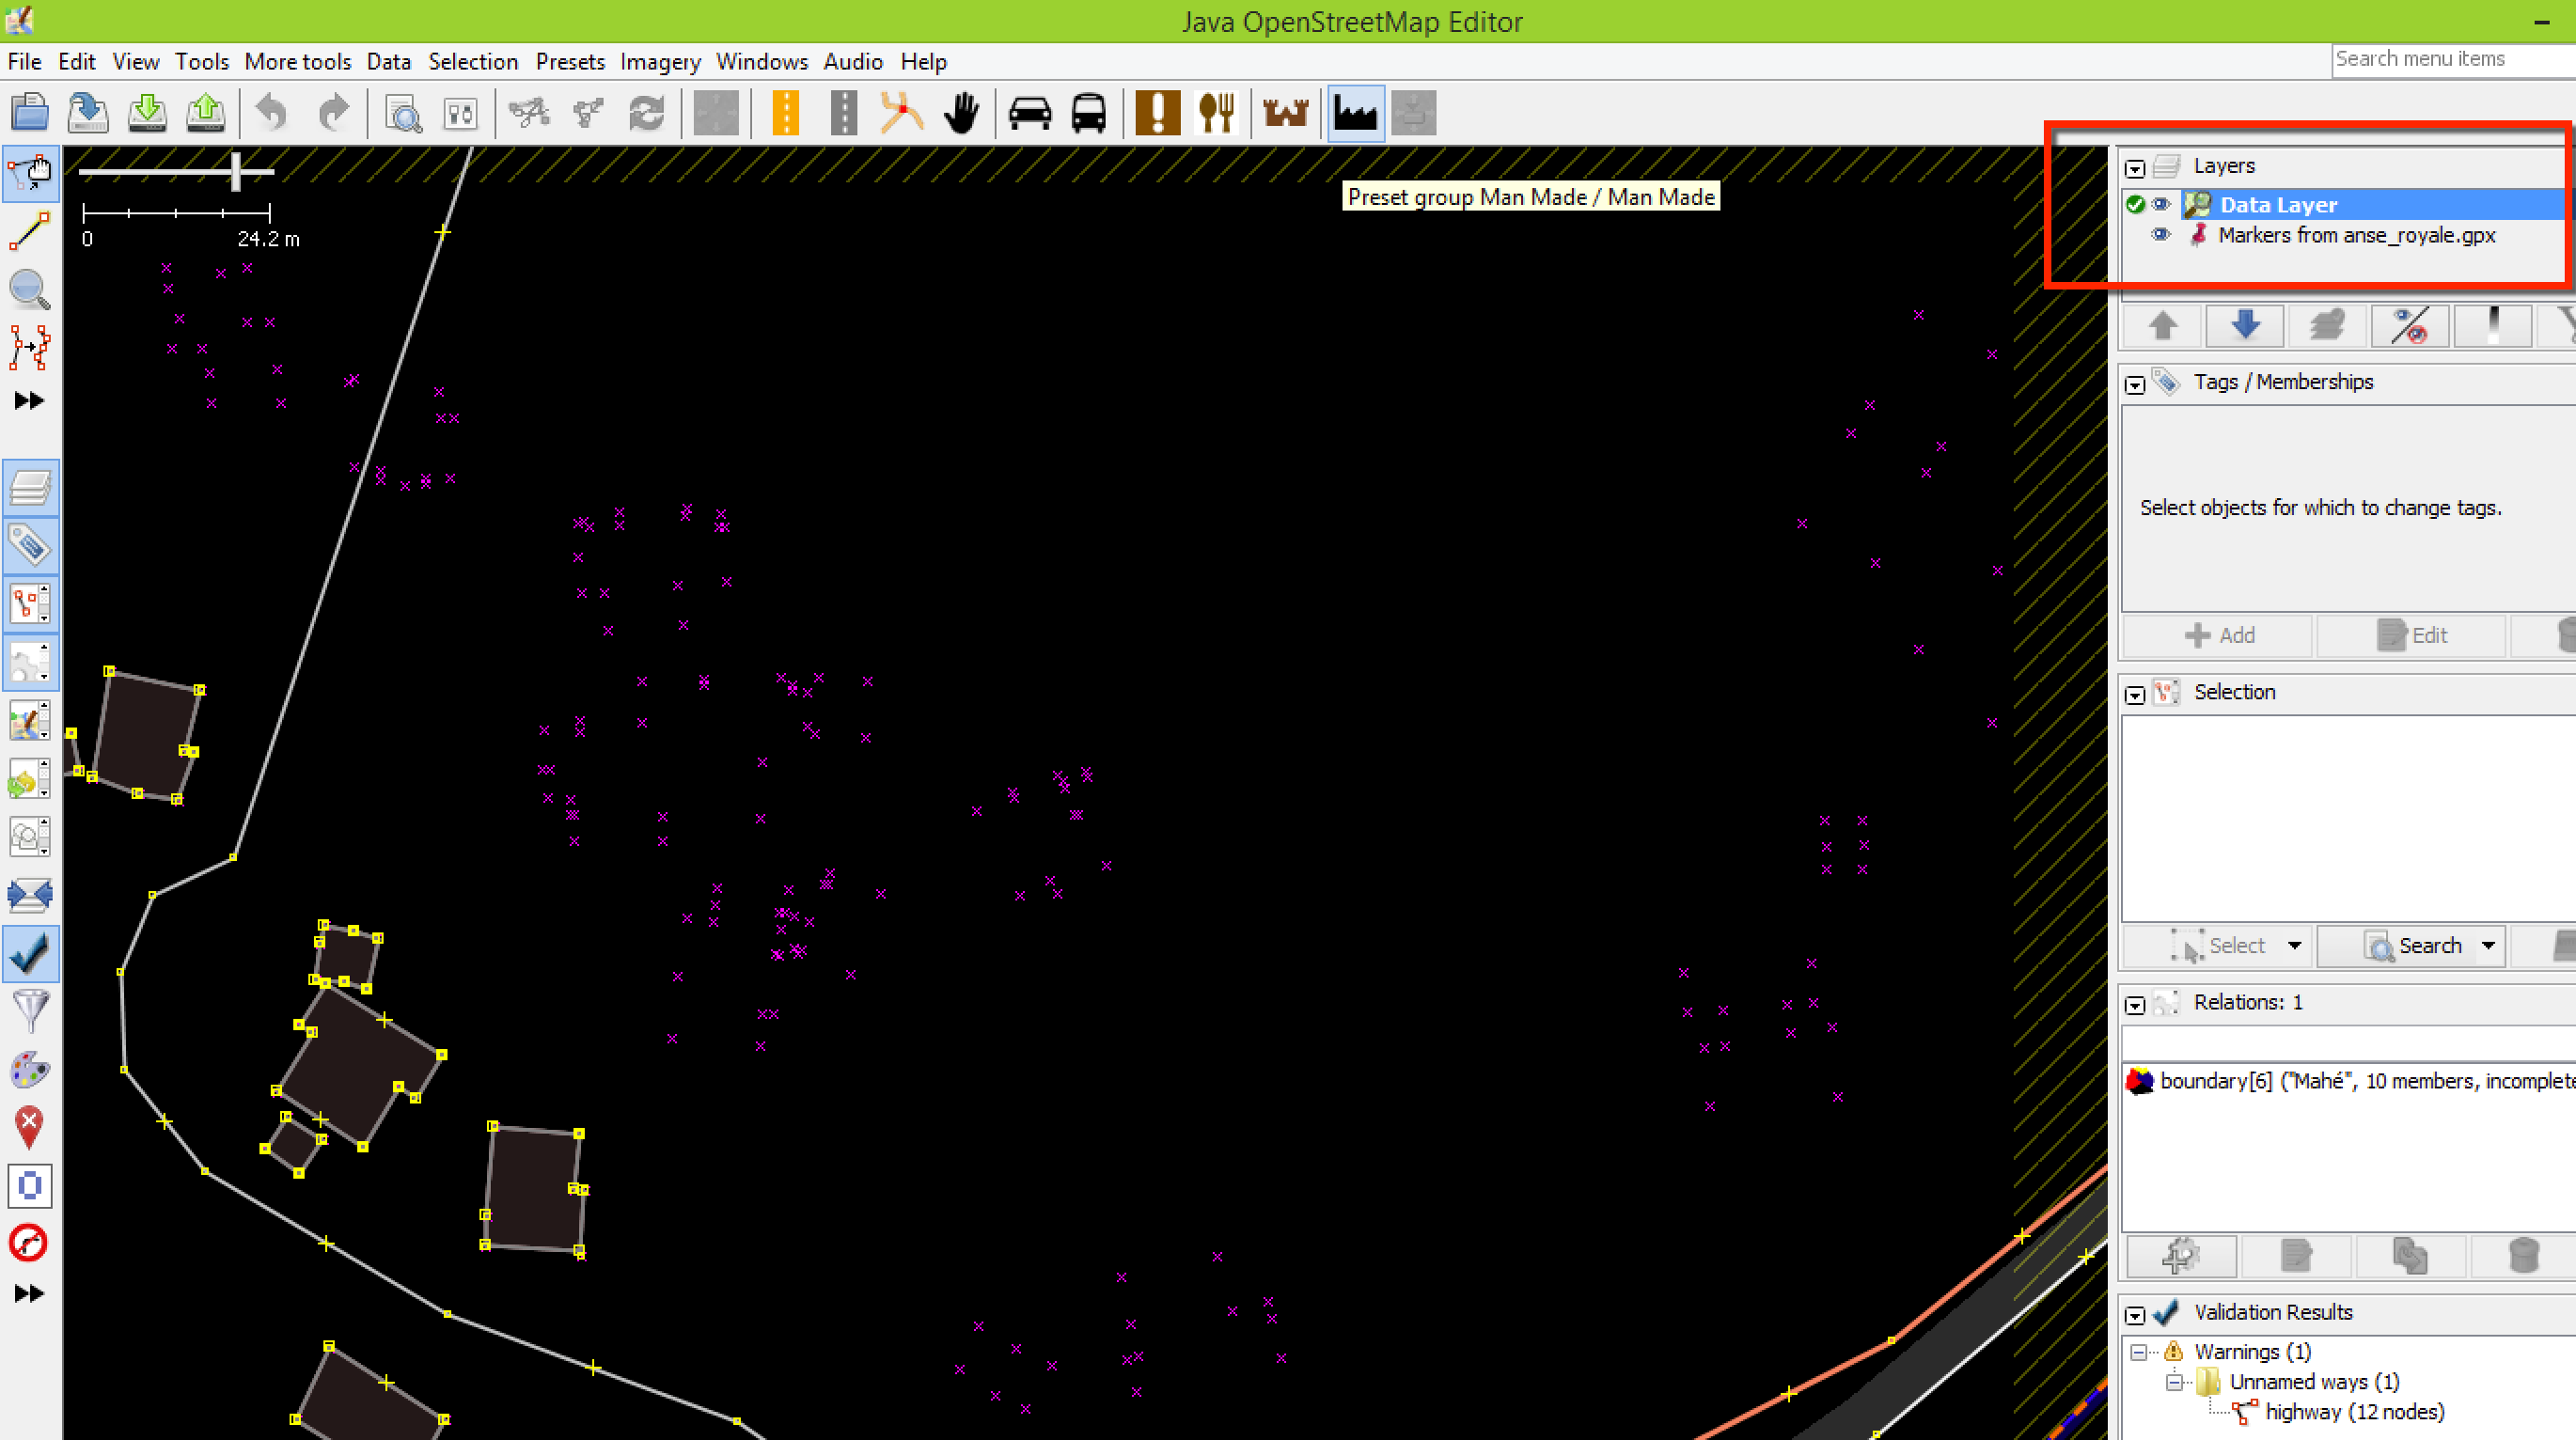
\includegraphics[width=12cm]{Images/load_gpx_file_3.png}
	\caption{OSM data layer and GPX layer}\label{fig:load_gpx_3}
\end{figure}

To be able to edit the GPX layer you have to convert it to a \textit{Data Layer}. This can be done through the context menu of the GPX layer (Figure \ref{fig:load_gpx_4}). Converting the layer will automatically set it as the active layer.

\begin{figure}[H]
	\centering
	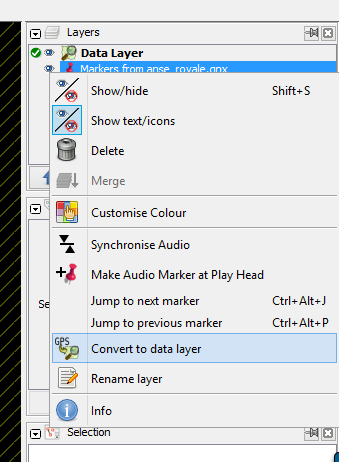
\includegraphics[width=8cm]{Images/load_gpx_file_4.png}
	\caption{Converting a GPX layer to a data layer}\label{fig:load_gpx_4}
\end{figure}

You can now use JOSM's \textit{Draw Nodes} tool to connect your nodes (waypoints) and create closed ways representing the building footprints (Figure \ref{fig:load_gpx_5}). You can add one of several image layers from a map service such as Bing, MapBox, etc. (through the \textit{Imagery} menu) that might give you a better idea how the surroundings of your working area looks like. Be aware that images from these services often have a shift and will not fit exactly with your data. Usually your own records (and imagery) will be more accurate, so you should rely on those primarily. 

\begin{figure}[H]
	\centering
	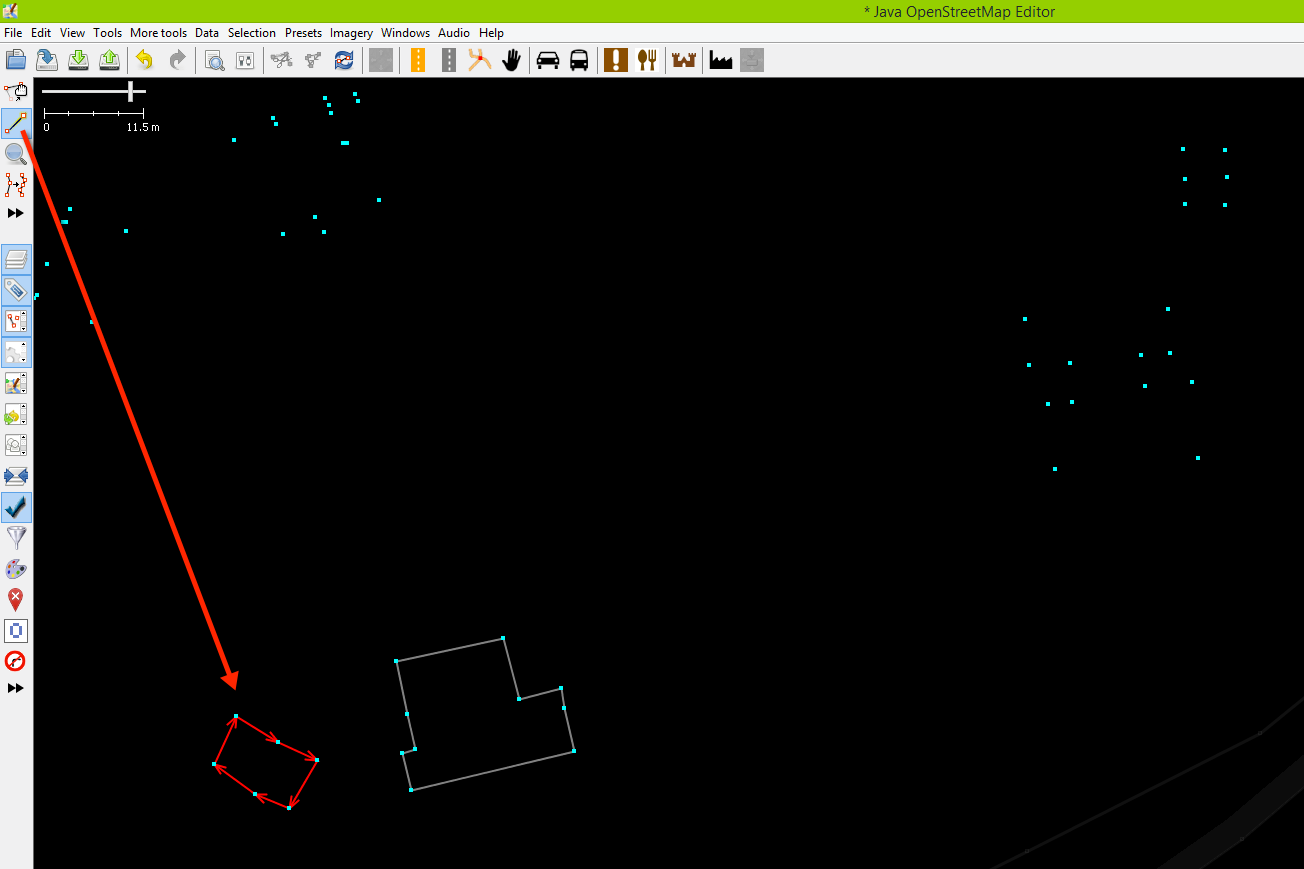
\includegraphics[width=12cm]{Images/load_gpx_file_5.png}
	\caption{Using the Draw Nodes tool to create building footprints}\label{fig:load_gpx_5}
\end{figure}

Once you created the building footprints you should properly tag the buildings to provide basic characteristics that will be useful for the other organisations and potentially for everyone else. A list of tags you should make use of is shown in Figure \ref{fig:building_tags}. This should be the amount of information you provide for each building you create (as far as you have that information available). For their own use organisations can later on add additional information that is relevant only to their work (once they have downloaded OSM data into their GIS software).

\begin{figure}[H]
	\centering
	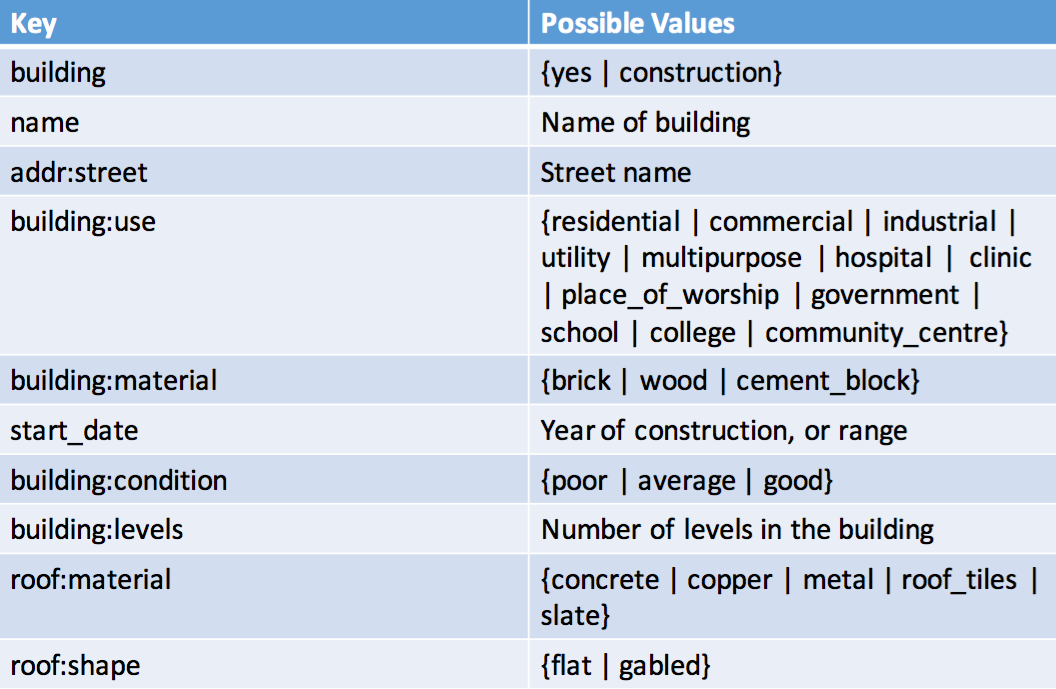
\includegraphics[width=12cm]{Images/building_tags.png}
	\caption{Basic building tags to be assigned}\label{fig:building_tags}
\end{figure}

To tag a building activate JOSM's \textit{Select} tool and select one or more buildings you want to tag. JOSM will offer you a list of common and previously used tags (Figure \ref{fig:building_tags_2}).

\begin{figure}[H]
	\centering
	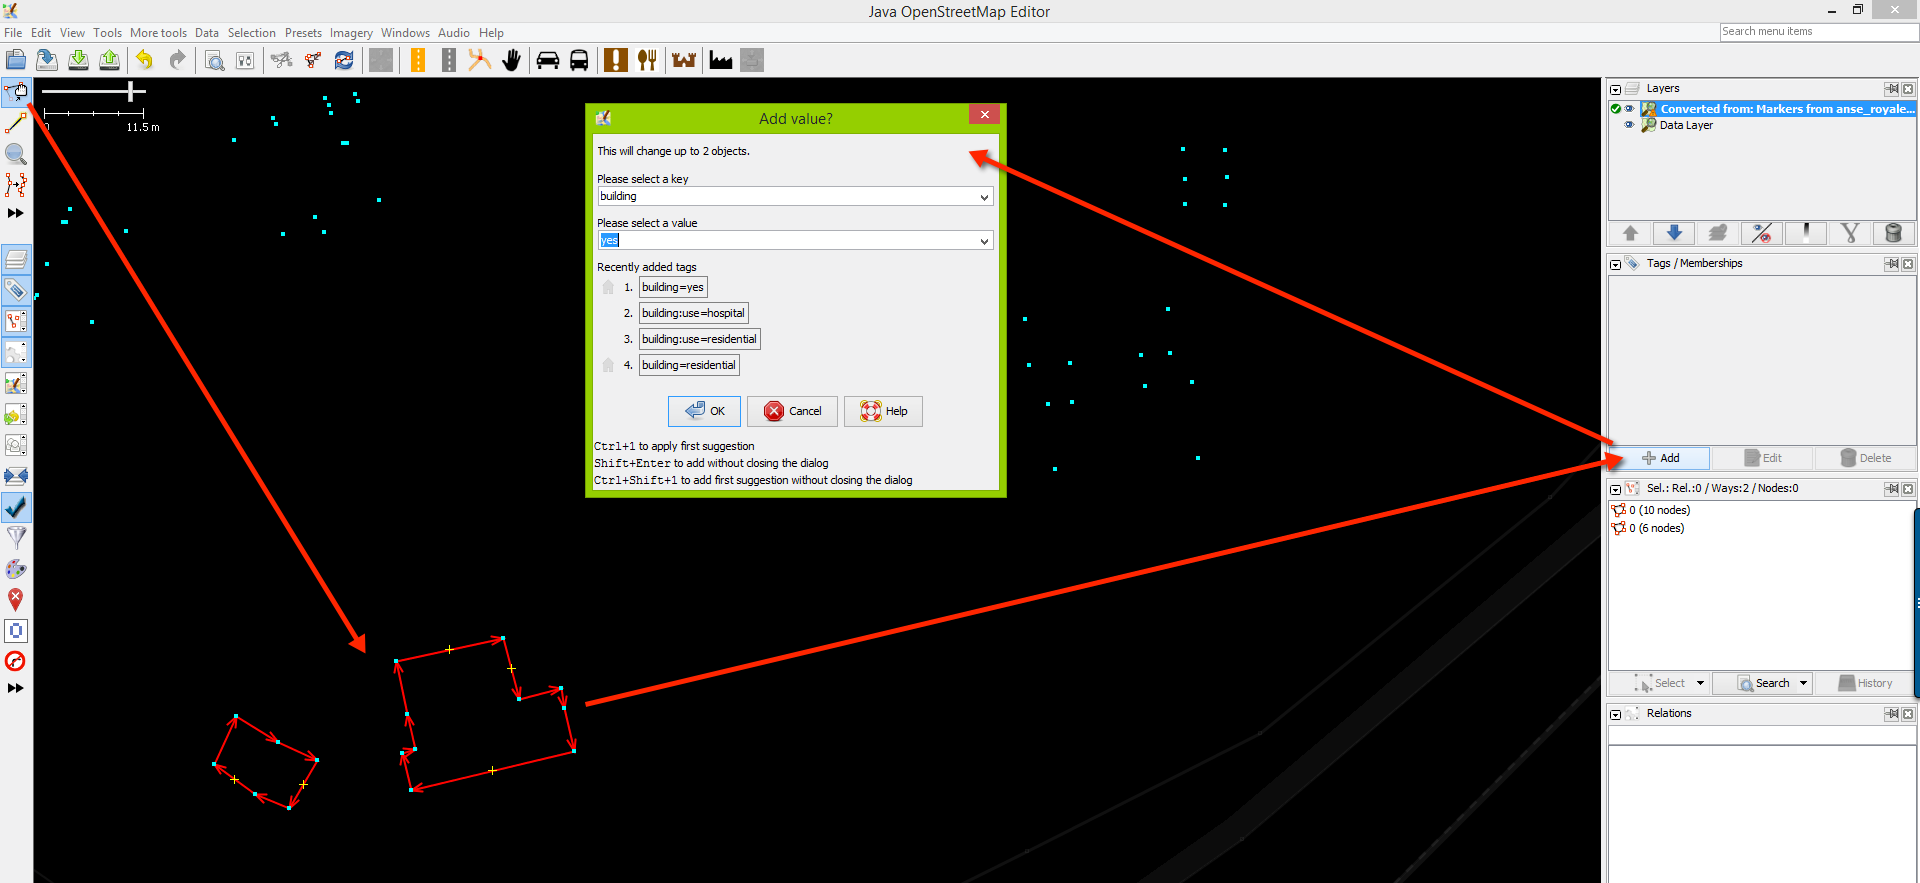
\includegraphics[width=12cm]{Images/building_tags_2.png}
	\caption{Assigning a tag}\label{fig:building_tags_2}
\end{figure}

In the example the two buildings were assigned two tags each (Figure \ref{fig:building_tags_3}).

\begin{figure}[H]
	\centering
	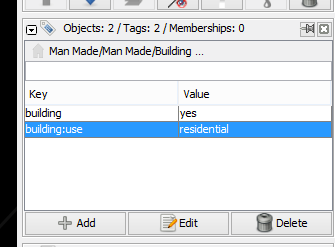
\includegraphics[width=8cm]{Images/building_tags_3.png}
	\caption{Assigned tags}\label{fig:building_tags_3}
\end{figure}

\section{Uploading your additions/changes to the OSM server}

Once you finished creating the building footprints and assigning the tags you should merge your data into the data layer containing the existing OSM data (that you previously downloaded). To do this select the buildings you want to merge and select \textit{Merge selection} from the \textit{Edit} menu. Select \textit{Data Layer} as the layer to merge into (Figure \ref{fig:merge_layers}). 

\begin{figure}[H]
	\centering
	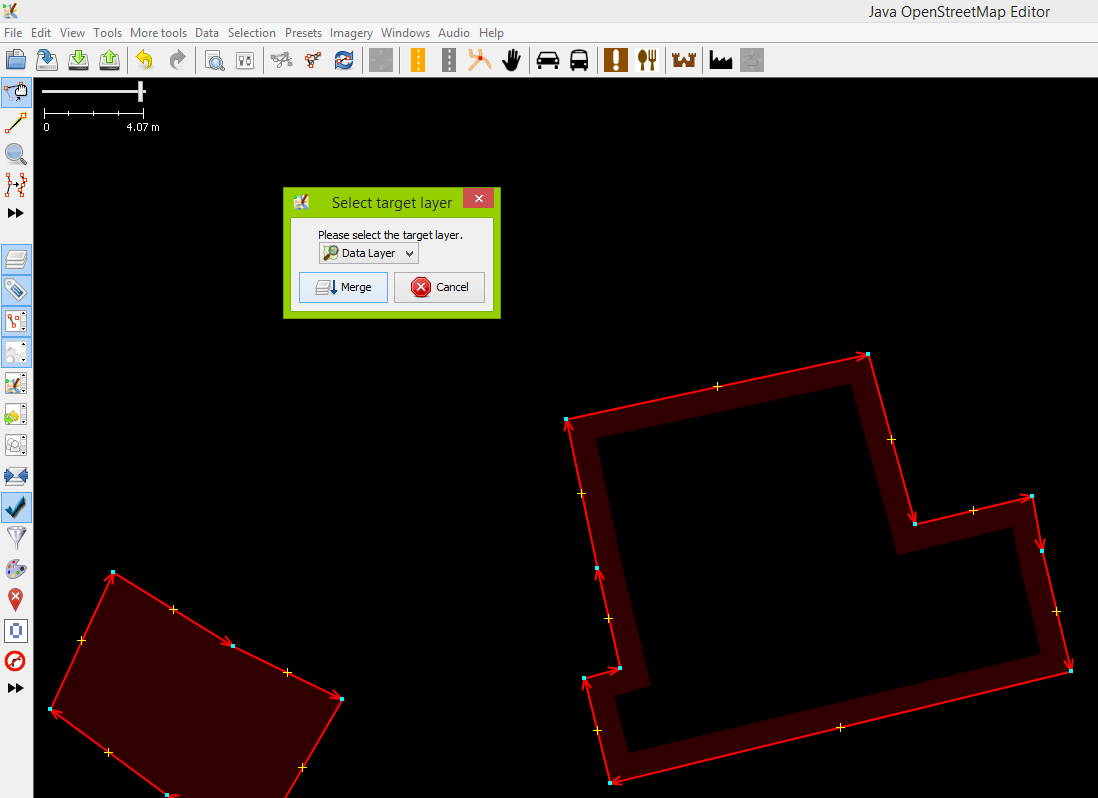
\includegraphics[width=12cm]{Images/merge_layers.png}
	\caption{Merging layers}\label{fig:merge_layers}
\end{figure}

After the merge make the \textit{Data Layer} the active layer (through the context menu). Click the \textit{Upload} tool to upload all changes in the active data layer to the OSM server. You will get a warning regarding the nodes of your buildings related to a tag \textit{name} that was assigned by JOSM when converting the GPX layer to a data layer (Figure \ref{fig:node_error}). The \textit{name} tag is not required here and should be removed before the upload. Cancel the upload for now. To fix that issue draw a selection window over the buildings you created. This will select all ways and nodes. We need to select only the nodes to be able to remove the \textit{name} tag. Click the \textit{Search} button of the \textit{Selection} window, type \textit{child selected} and click \textit{Start Search} (Figure \ref{fig:find_nodes}). As a result only the nodes will be selected.

\begin{figure}[H]
	\centering
	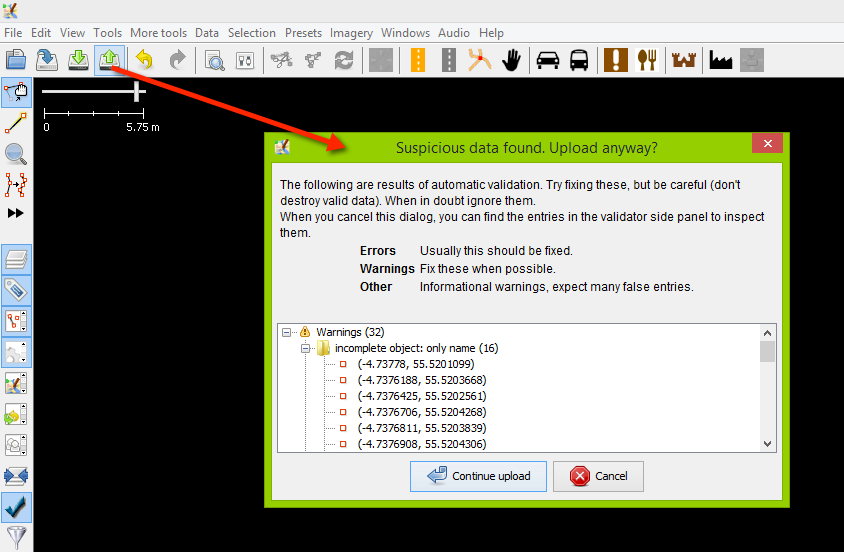
\includegraphics[width=12cm]{Images/node_error.png}
	\caption{1st upload attempt}\label{fig:node_error}
\end{figure}

\begin{figure}[H]
	\centering
	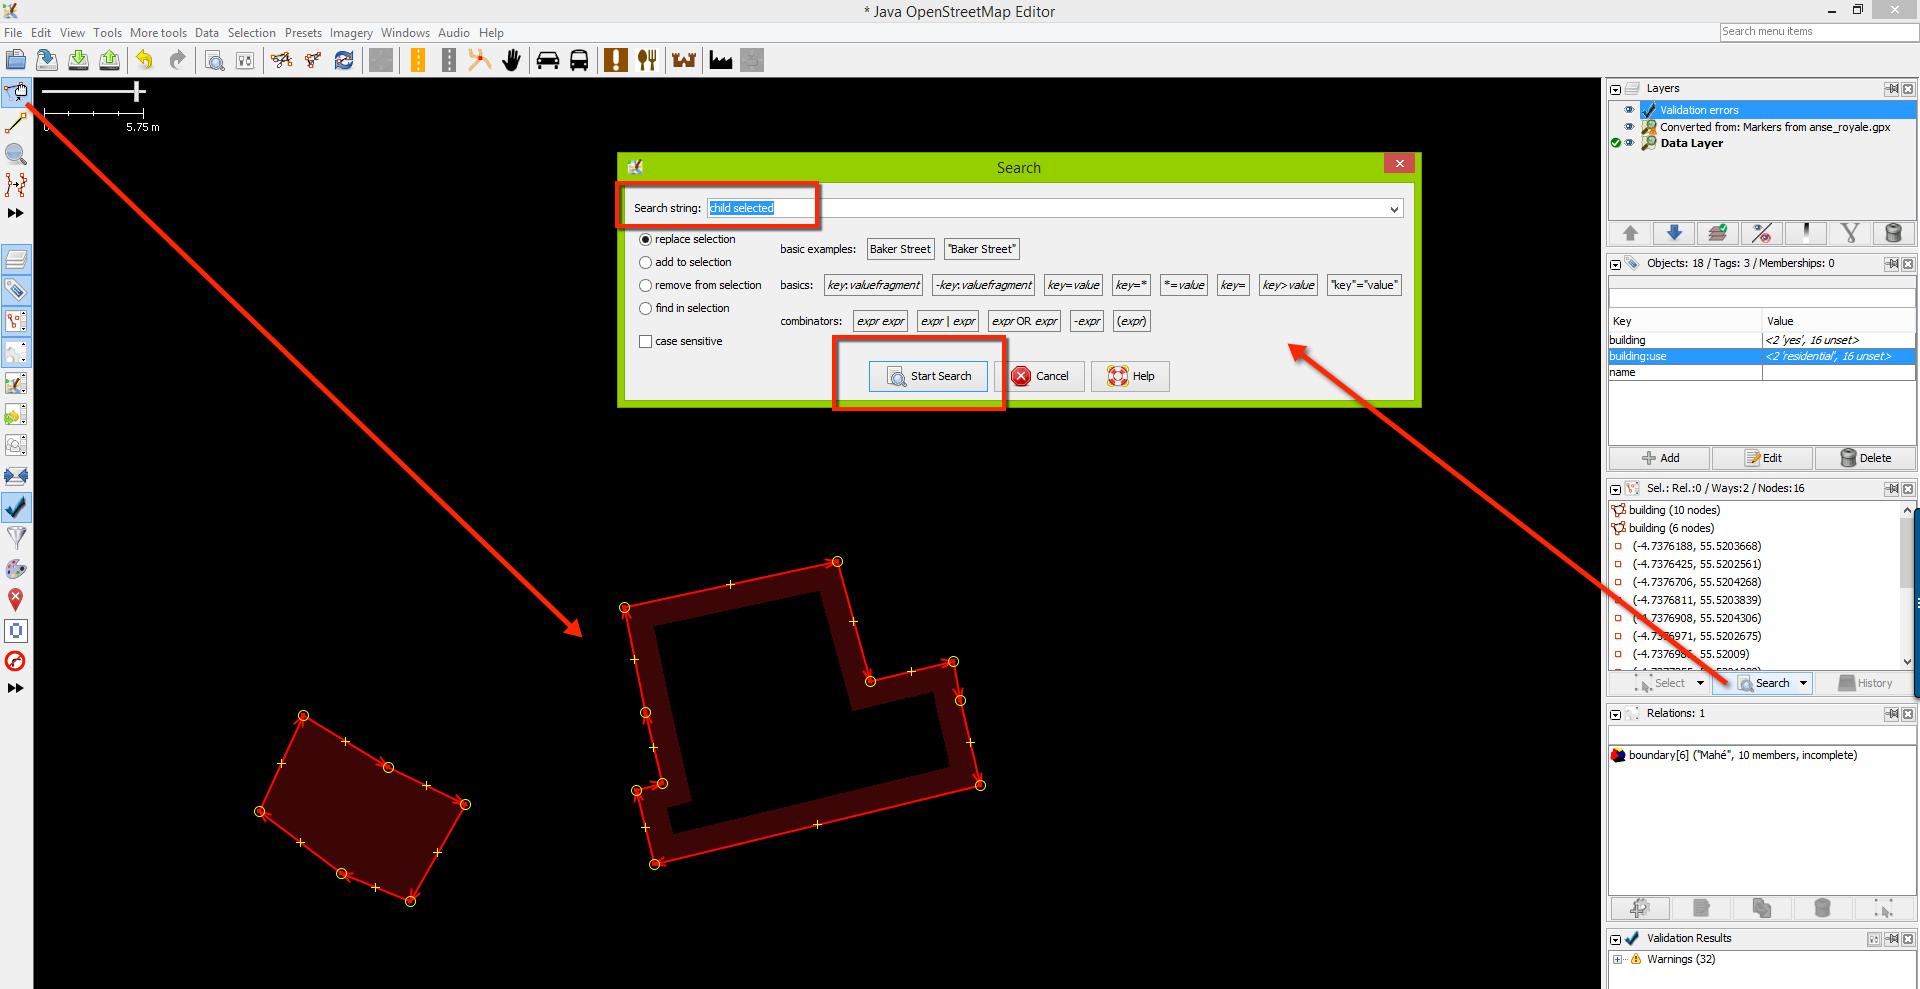
\includegraphics[width=12cm]{Images/find_nodes.png}
	\caption{Select nodes only}\label{fig:find_nodes}
\end{figure}

Click the \textit{Delete} button in the \textit{Tags/Memberships} window to remove the \textit{name} tag from all nodes at once (Figure \ref{fig:remove_tag}). Click the Upload button again, this time no warning should be shown anymore. In the resulting dialog window provide a brief description of your additions or changes and click the \textit{Upload Changes} button (Figure \ref{fig:upload_attempt_2}). Your data should successfully upload to the OSM server. You can verify that by browsing to the area of your changes on \url{www.openstreetmap.org}. The new buildings should be shown there.

\begin{figure}[H]
	\centering
	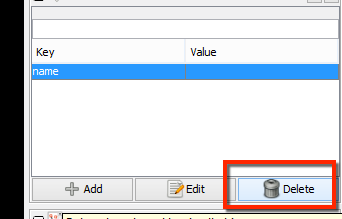
\includegraphics[width=8cm]{Images/remove_tag.png}
	\caption{Remove \textit{name} tag from nodes}\label{fig:remove_tag}
\end{figure}

\begin{figure}[H]
	\centering
	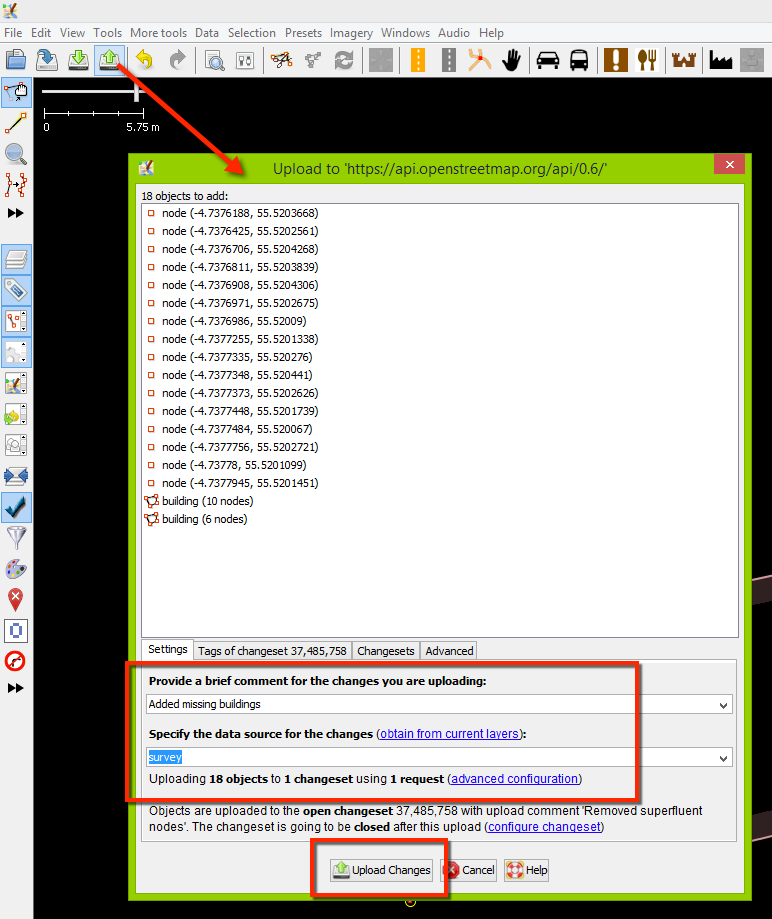
\includegraphics[width=8cm]{Images/upload_attempt_2.png}
	\caption{Description of changes before upload}\label{fig:upload_attempt_2}
\end{figure}

\section{Workflow to upload data from Shapefiles}

Quite often you might have created building footprints and relating attributes with the GIS software used by your organisation. If you want to contribute these buildings to OSM the workflow is slightly different from the one described previously (using GPX files). Once you are done with your edits you would select the buildings to be uploaded to OSM later on and export them to a Shapefile (using WGS84, EPSG-ID:4326 as coordinate reference system). How this is done depends on your particular GIS software. In this guideline it is shown how it can be done using QGIS. Figure \ref{fig:qgis_1} shows a database layer with building information (\textit{sv\_building}).

\begin{figure}[H]
	\centering
	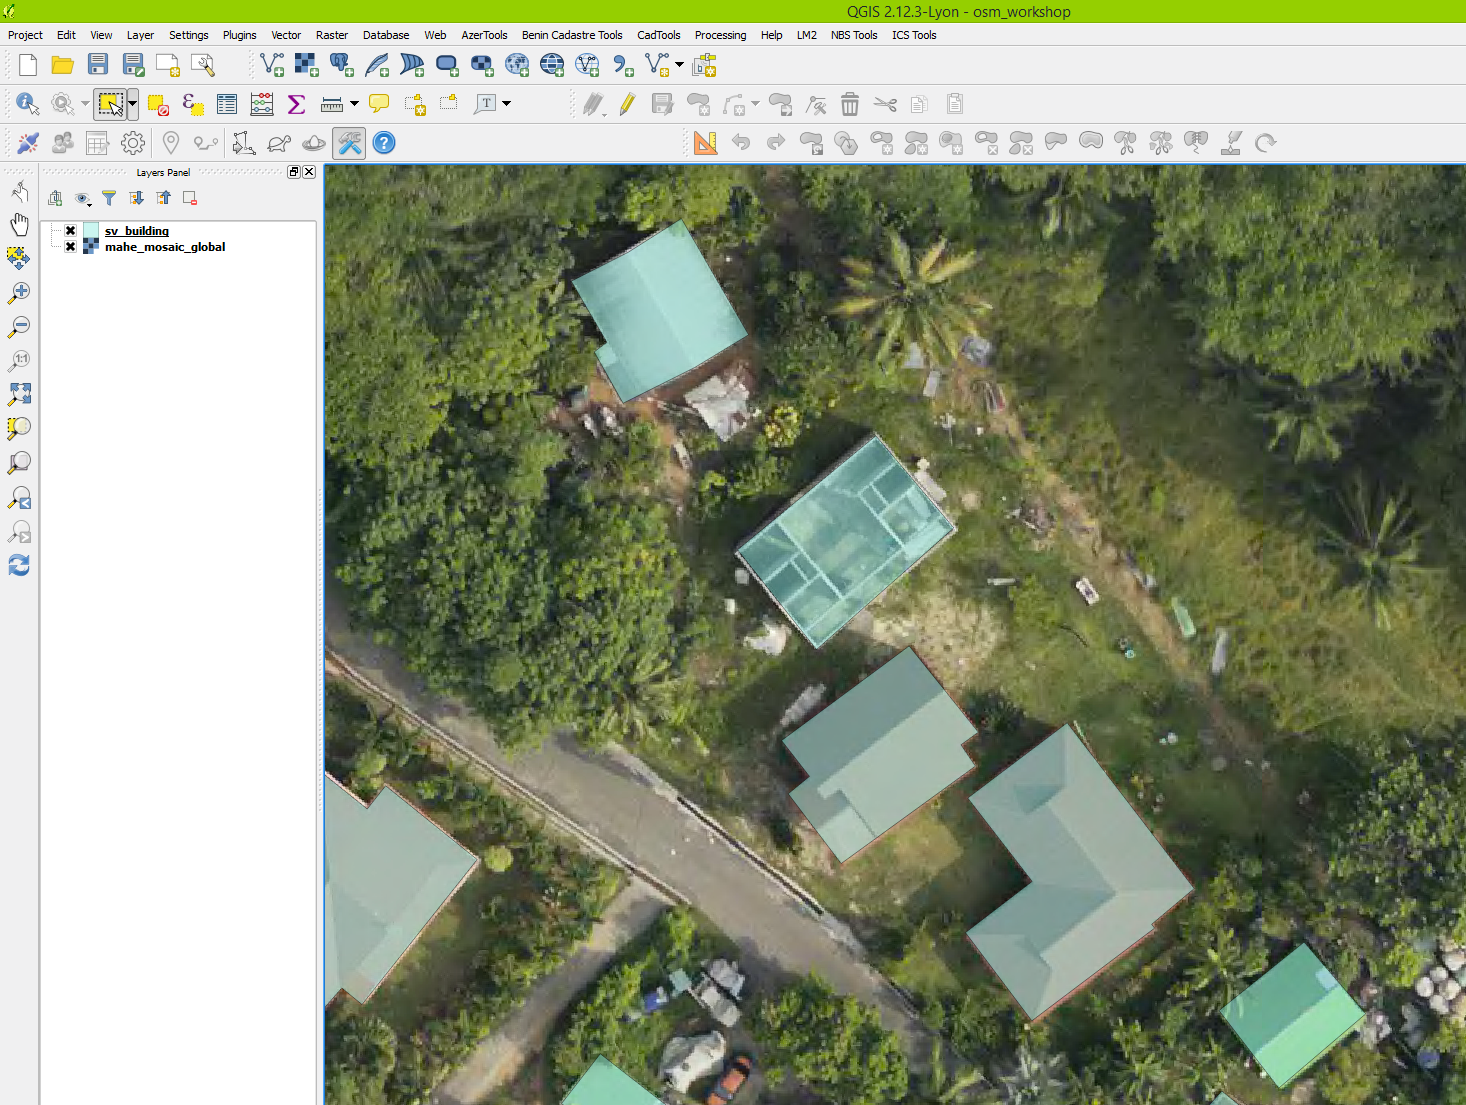
\includegraphics[width=12cm]{Images/qgis_1.png}
	\caption{Building layer in QGIS}\label{fig:qgis_1}
\end{figure}

To export the five buildings currently shown in the map extent select them with the QGIS selection tool and click \textit{Save As...} from the layer's context menu. In the resulting dialog do the settings as shown in Figure \ref{fig:qgis_2}.

\begin{figure}[H]
	\centering
	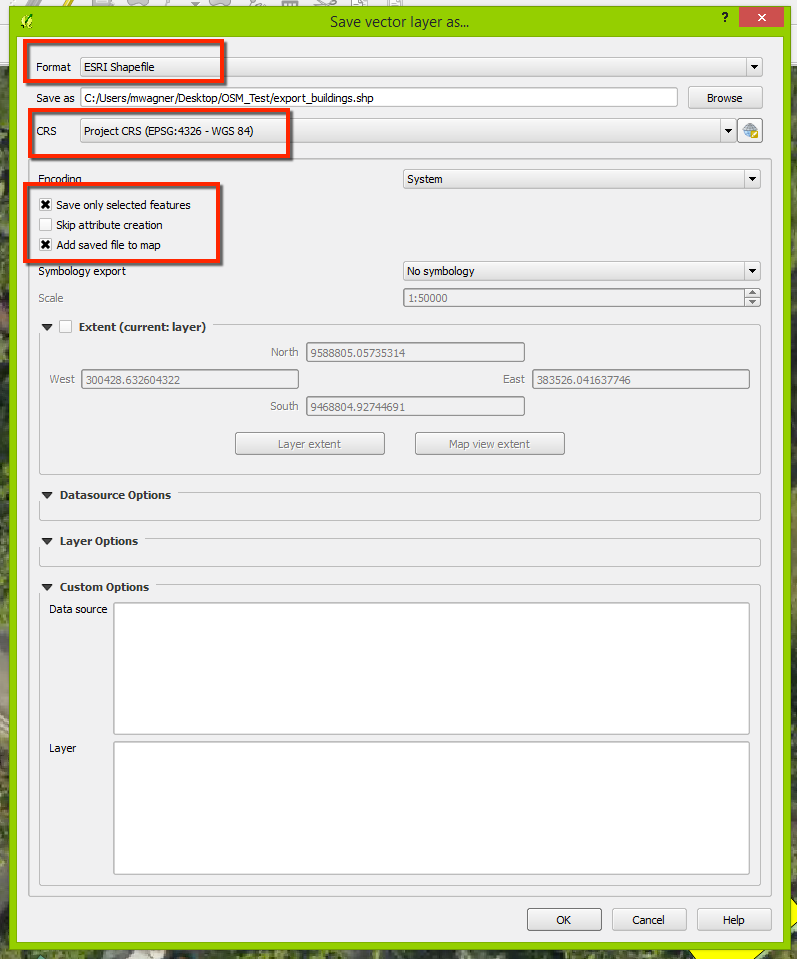
\includegraphics[width=8cm]{Images/qgis_2.png}
	\caption{Exported layer in QGIS}\label{fig:qgis_2}
\end{figure}

As a result the new Shapefile layer will be loaded into QGIS and should contain the five selected buildings only (Figure \ref{fig:qgis_3}). At this point you can quit QGIS and launch JOSM.

\begin{figure}[H]
	\centering
	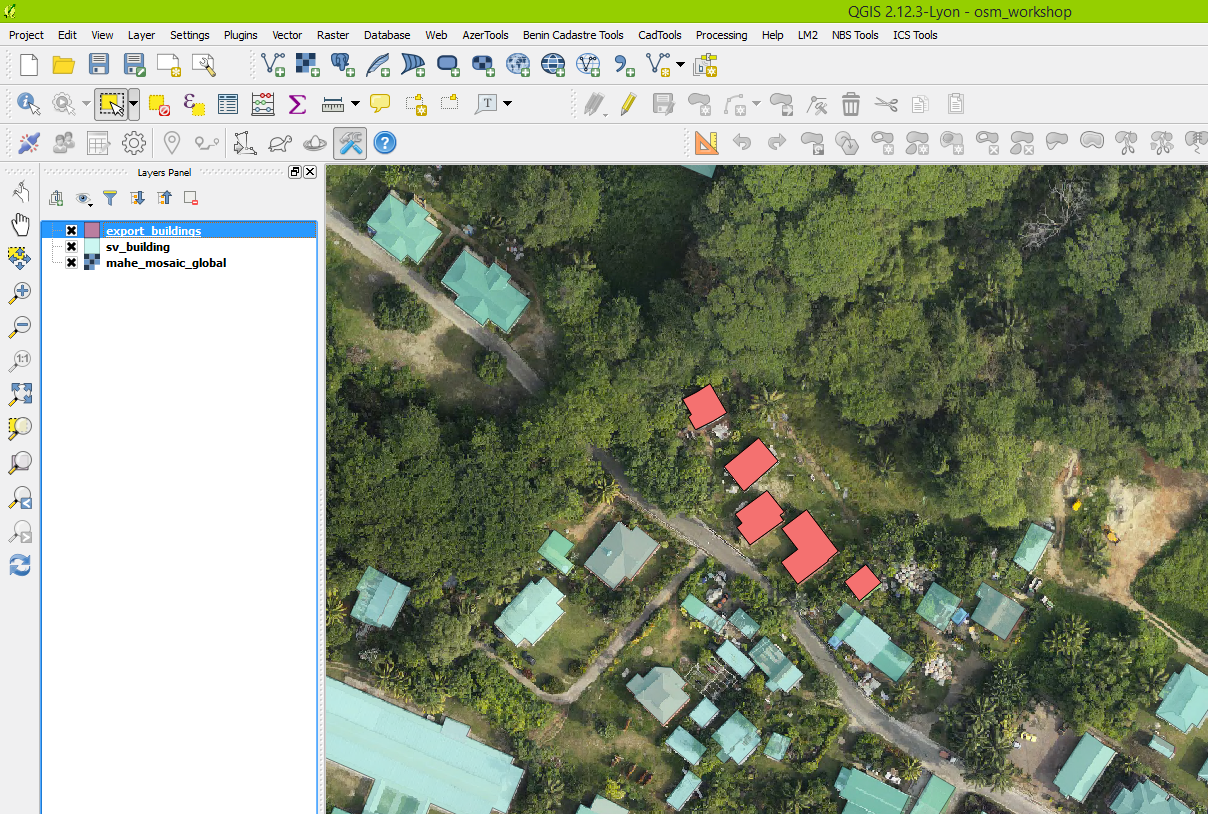
\includegraphics[width=12cm]{Images/qgis_3.png}
	\caption{Exported layer in QGIS}\label{fig:qgis_3}
\end{figure}

In JOSM load the exported Shapefile by selecting \textit{Open} from the \textit{File} menu. The result would look like Figure \ref{fig:josm_shape_1}.

\begin{figure}[H]
	\centering
	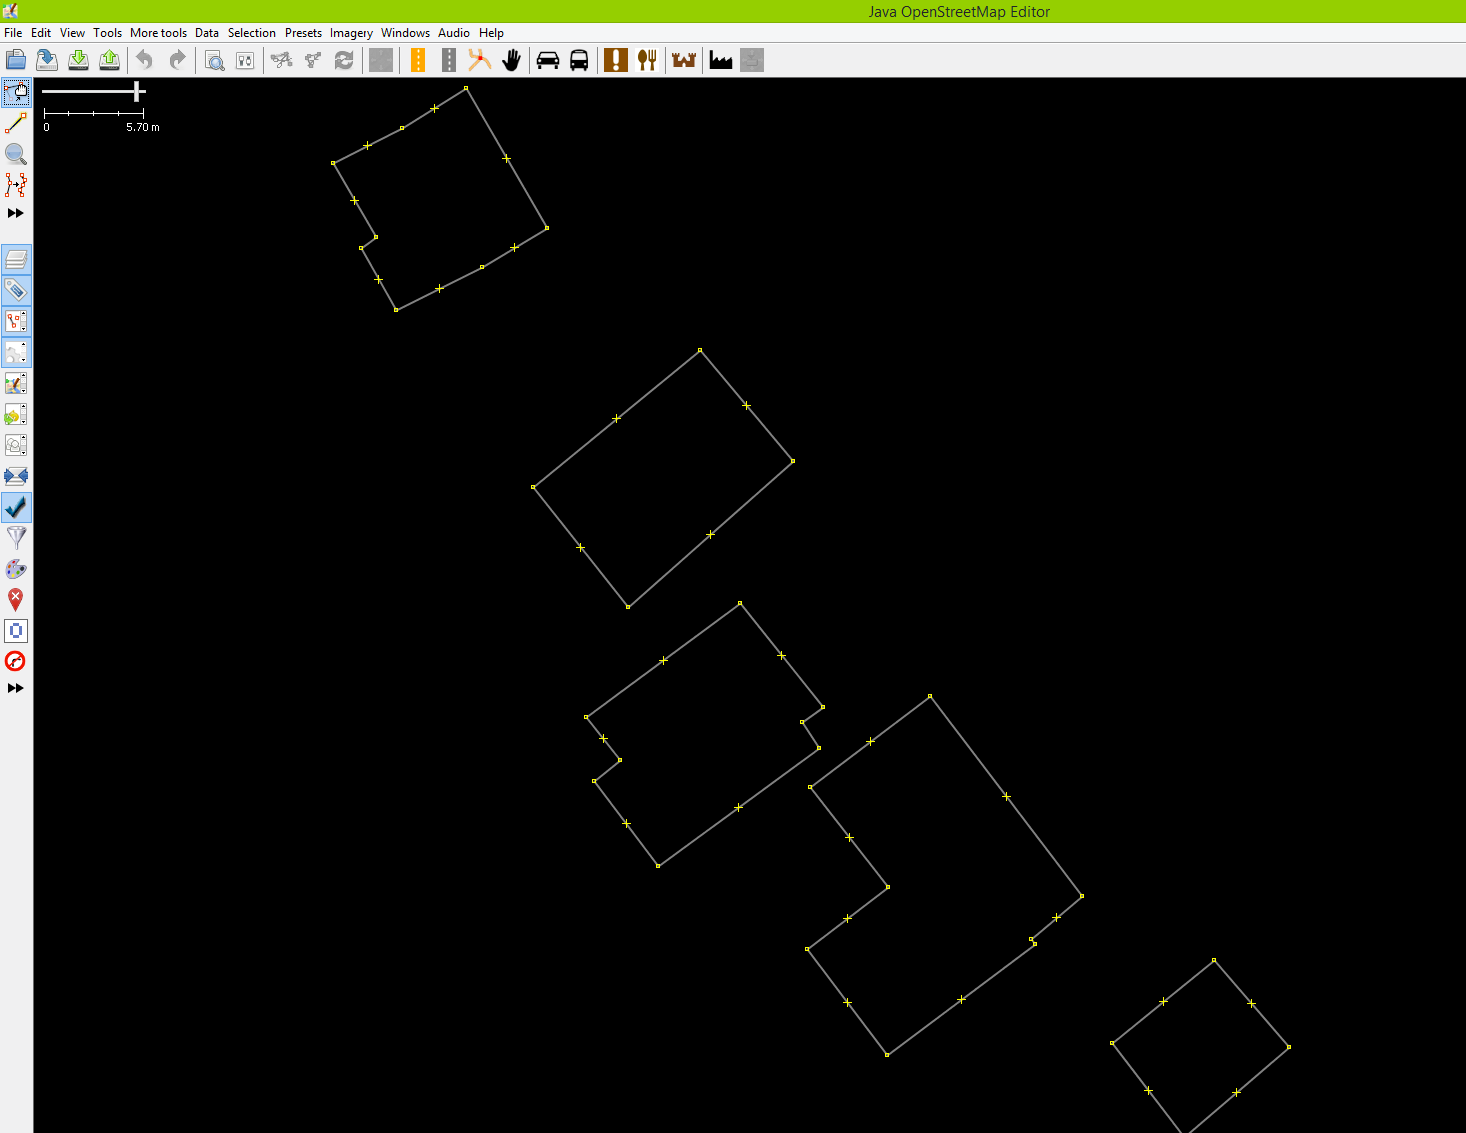
\includegraphics[width=12cm]{Images/josm_shape_1.png}
	\caption{Shapefile loaded into JOSM}\label{fig:josm_shape_1}
\end{figure}

Click the \textit{Download map data from the OSM server} button to download OSM data for the area you imported the Shapefile for. JOSM recognizes the extent of your Shapefile data and will automatically offer to download data for that area only (this is the same procedure as with the GPX file previously). Make sure to toggle the checkbox \textit{Download as new layer}. Select the buildings you want to merge and select \textit{Merge selection} from the \textit{Edit} menu. Select \textit{Data Layer 1} as the layer to merge into  (Figure \ref{fig:josm_shape_2}). Ignore the warning that will appear regarding the merge of more than one object.

\begin{figure}[H]
	\centering
	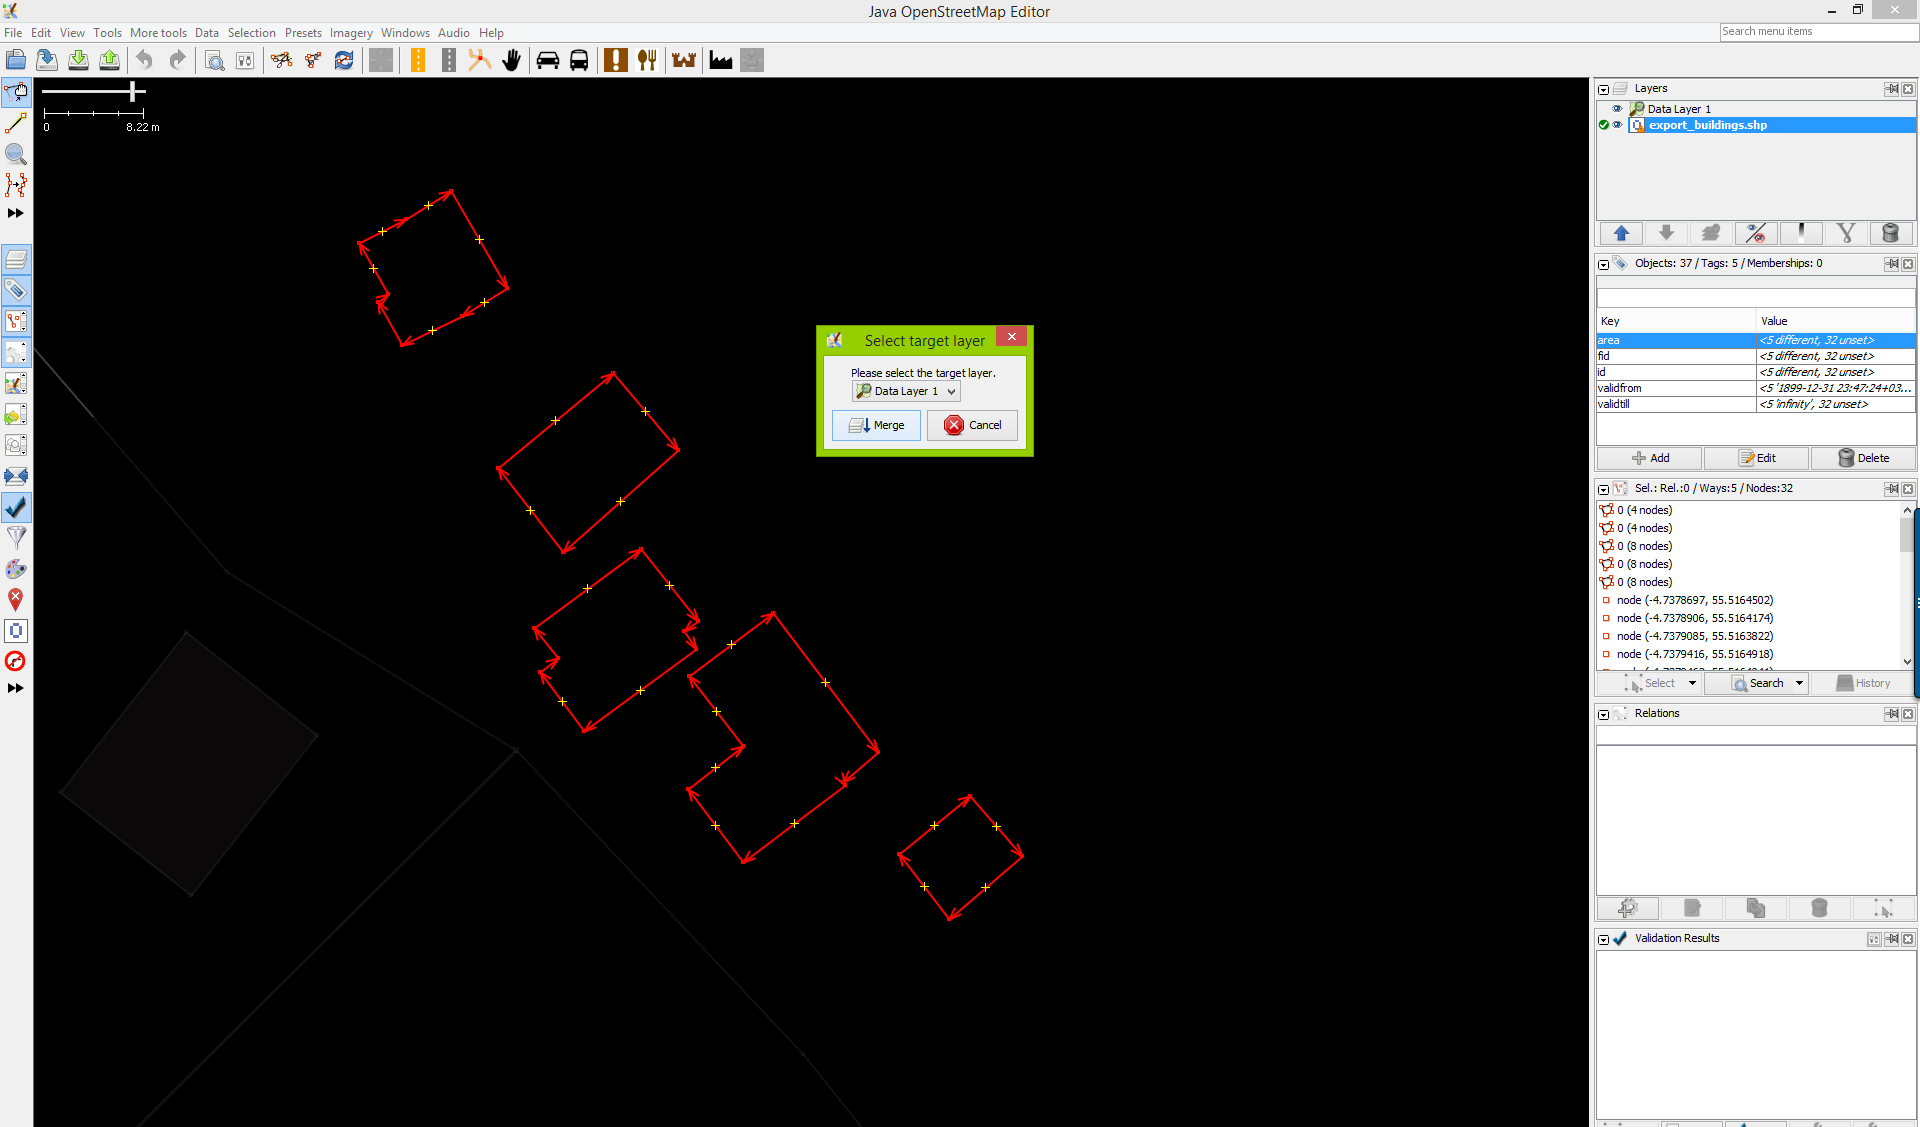
\includegraphics[width=12cm]{Images/josm_shape_2.png}
	\caption{Merging selected buildings into data layer}\label{fig:josm_shape_2}
\end{figure}

Make \textit{Data Layer 1} the active layer, the five buildings should appear in that layer now. These buildings have the attribute values from the original Shapefile assigned as tags. Select the five buildings and remove all current tags through the \textit{Tags/Memberships} window (Figure \ref{fig:josm_shape_3}).

\begin{figure}[H]
	\centering
	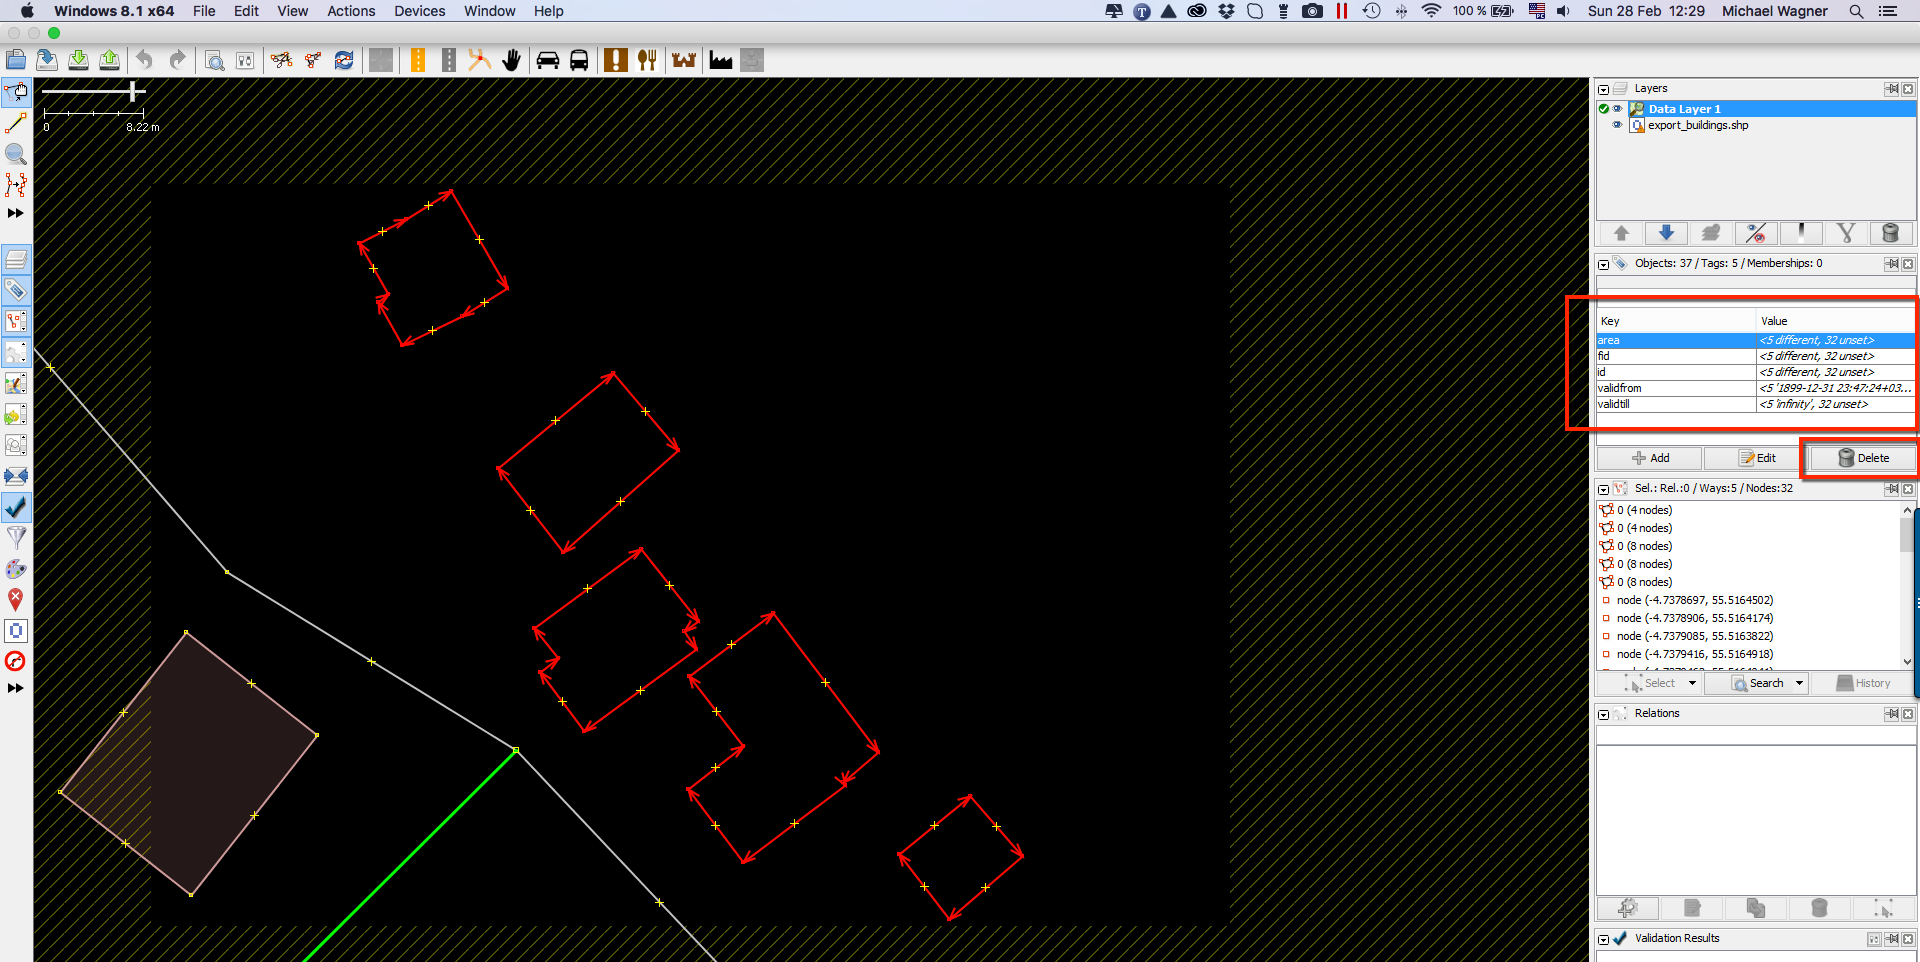
\includegraphics[width=12cm]{Images/josm_shape_3.png}
	\caption{Removing tags from selected buildings}\label{fig:josm_shape_3}
\end{figure}

Select one or multiple buildings and add the recommended tags as described previously for the GPX file import (Figure \ref{fig:josm_shape_4}).

\begin{figure}[H]
	\centering
	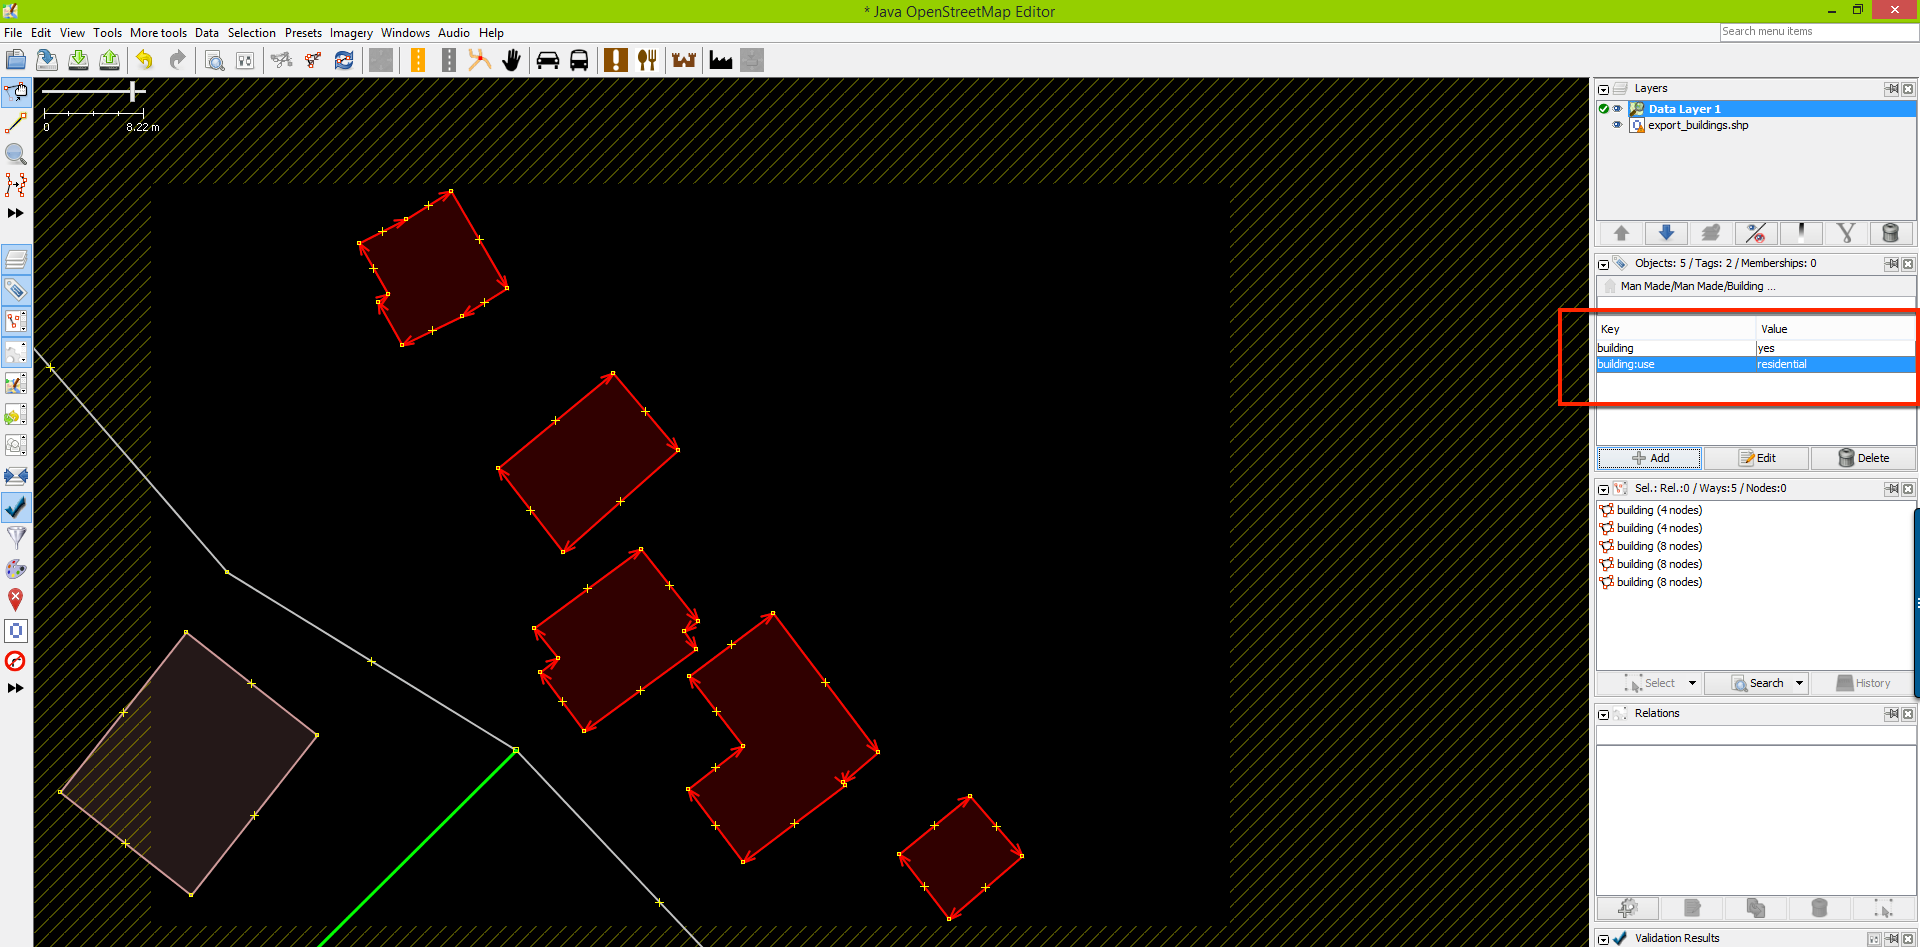
\includegraphics[width=12cm]{Images/josm_shape_4.png}
	\caption{Adding recommended tags to selected buildings}\label{fig:josm_shape_4}
\end{figure}

Click the \textit{Upload} button, add a brief description of your changes and upload the changes to the OSM server (Figure \ref{fig:josm_shape_5}). Verify a successful upload by browsing to your editing area on \url{www.openstreetmap.org}.

\begin{figure}[H]
	\centering
	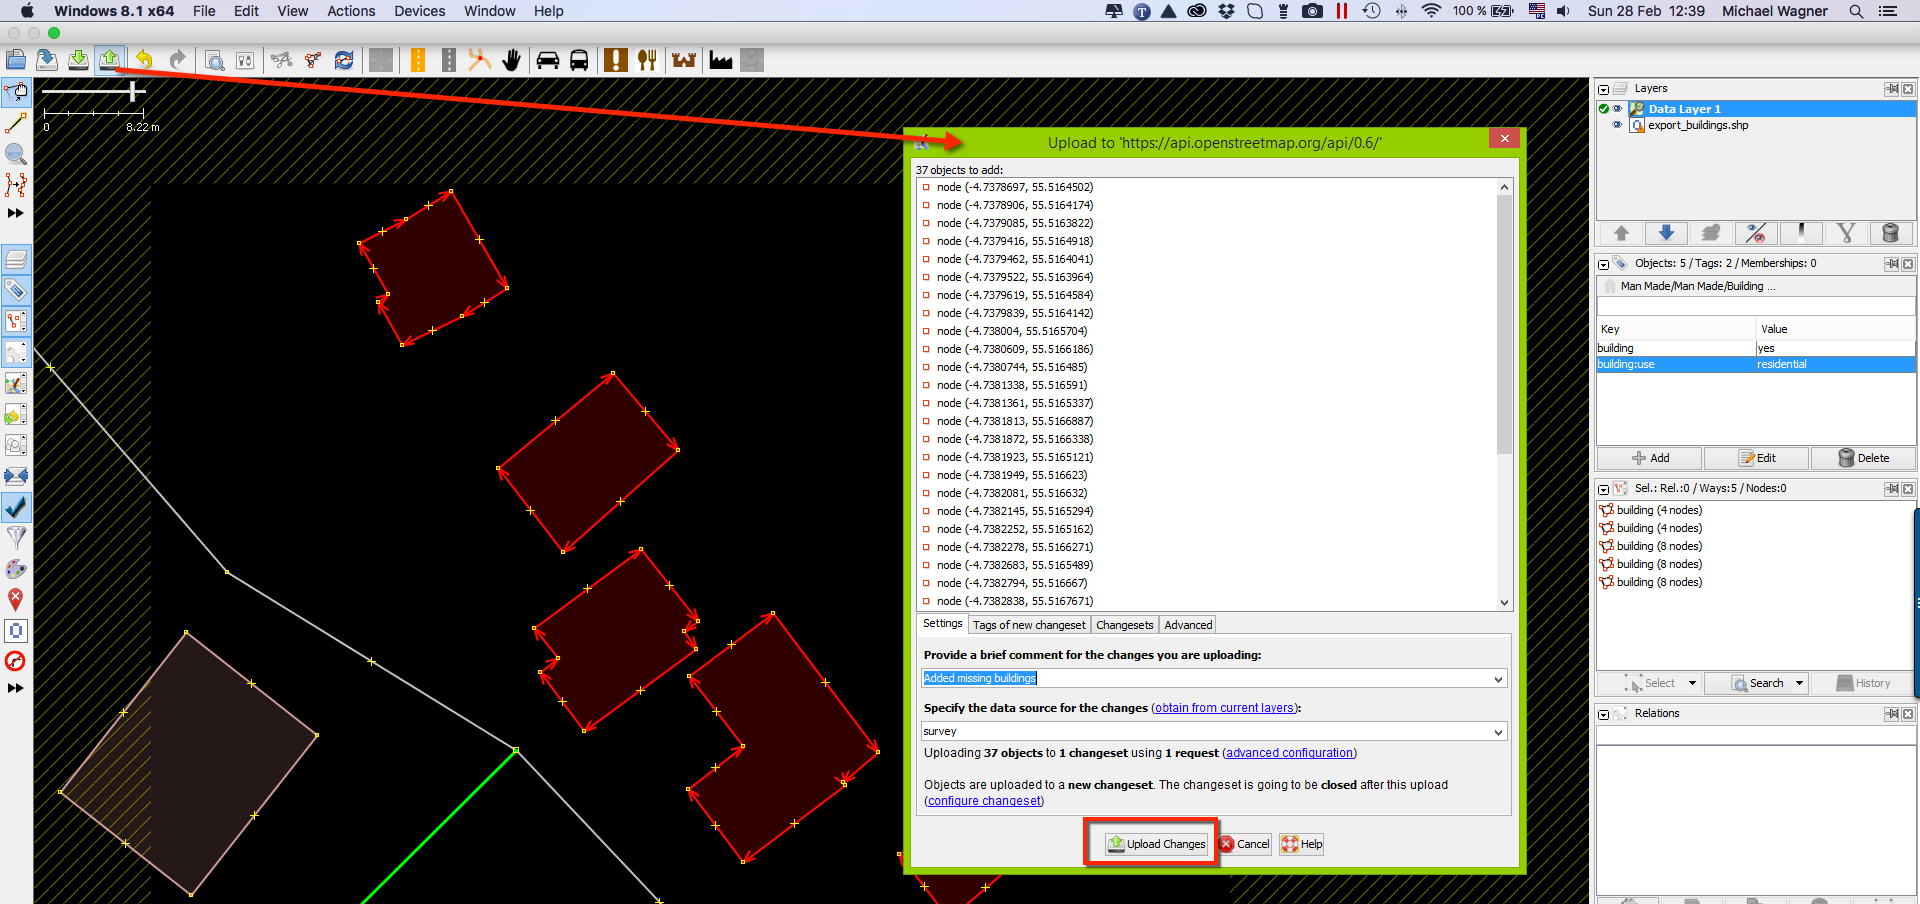
\includegraphics[width=12cm]{Images/josm_shape_5.png}
	\caption{Uploading changes to OSM server}\label{fig:josm_shape_5}
\end{figure}

\section{Downloading OSM data for use in QGIS}

At some point you might want to use OSM data in your own GIS software e.g. after another organisation has uploaded buildings that are still missing from your own building dataset. Loading this data into QGIS requires three main steps.

Browse and zoom to the area of interest on \url{www.openstreetmap.org}. Click \textit{Export} on the top-left side of the page and save the resulting *.osm file (Figure \ref{fig:import_1}).

\begin{figure}[H]
	\centering
	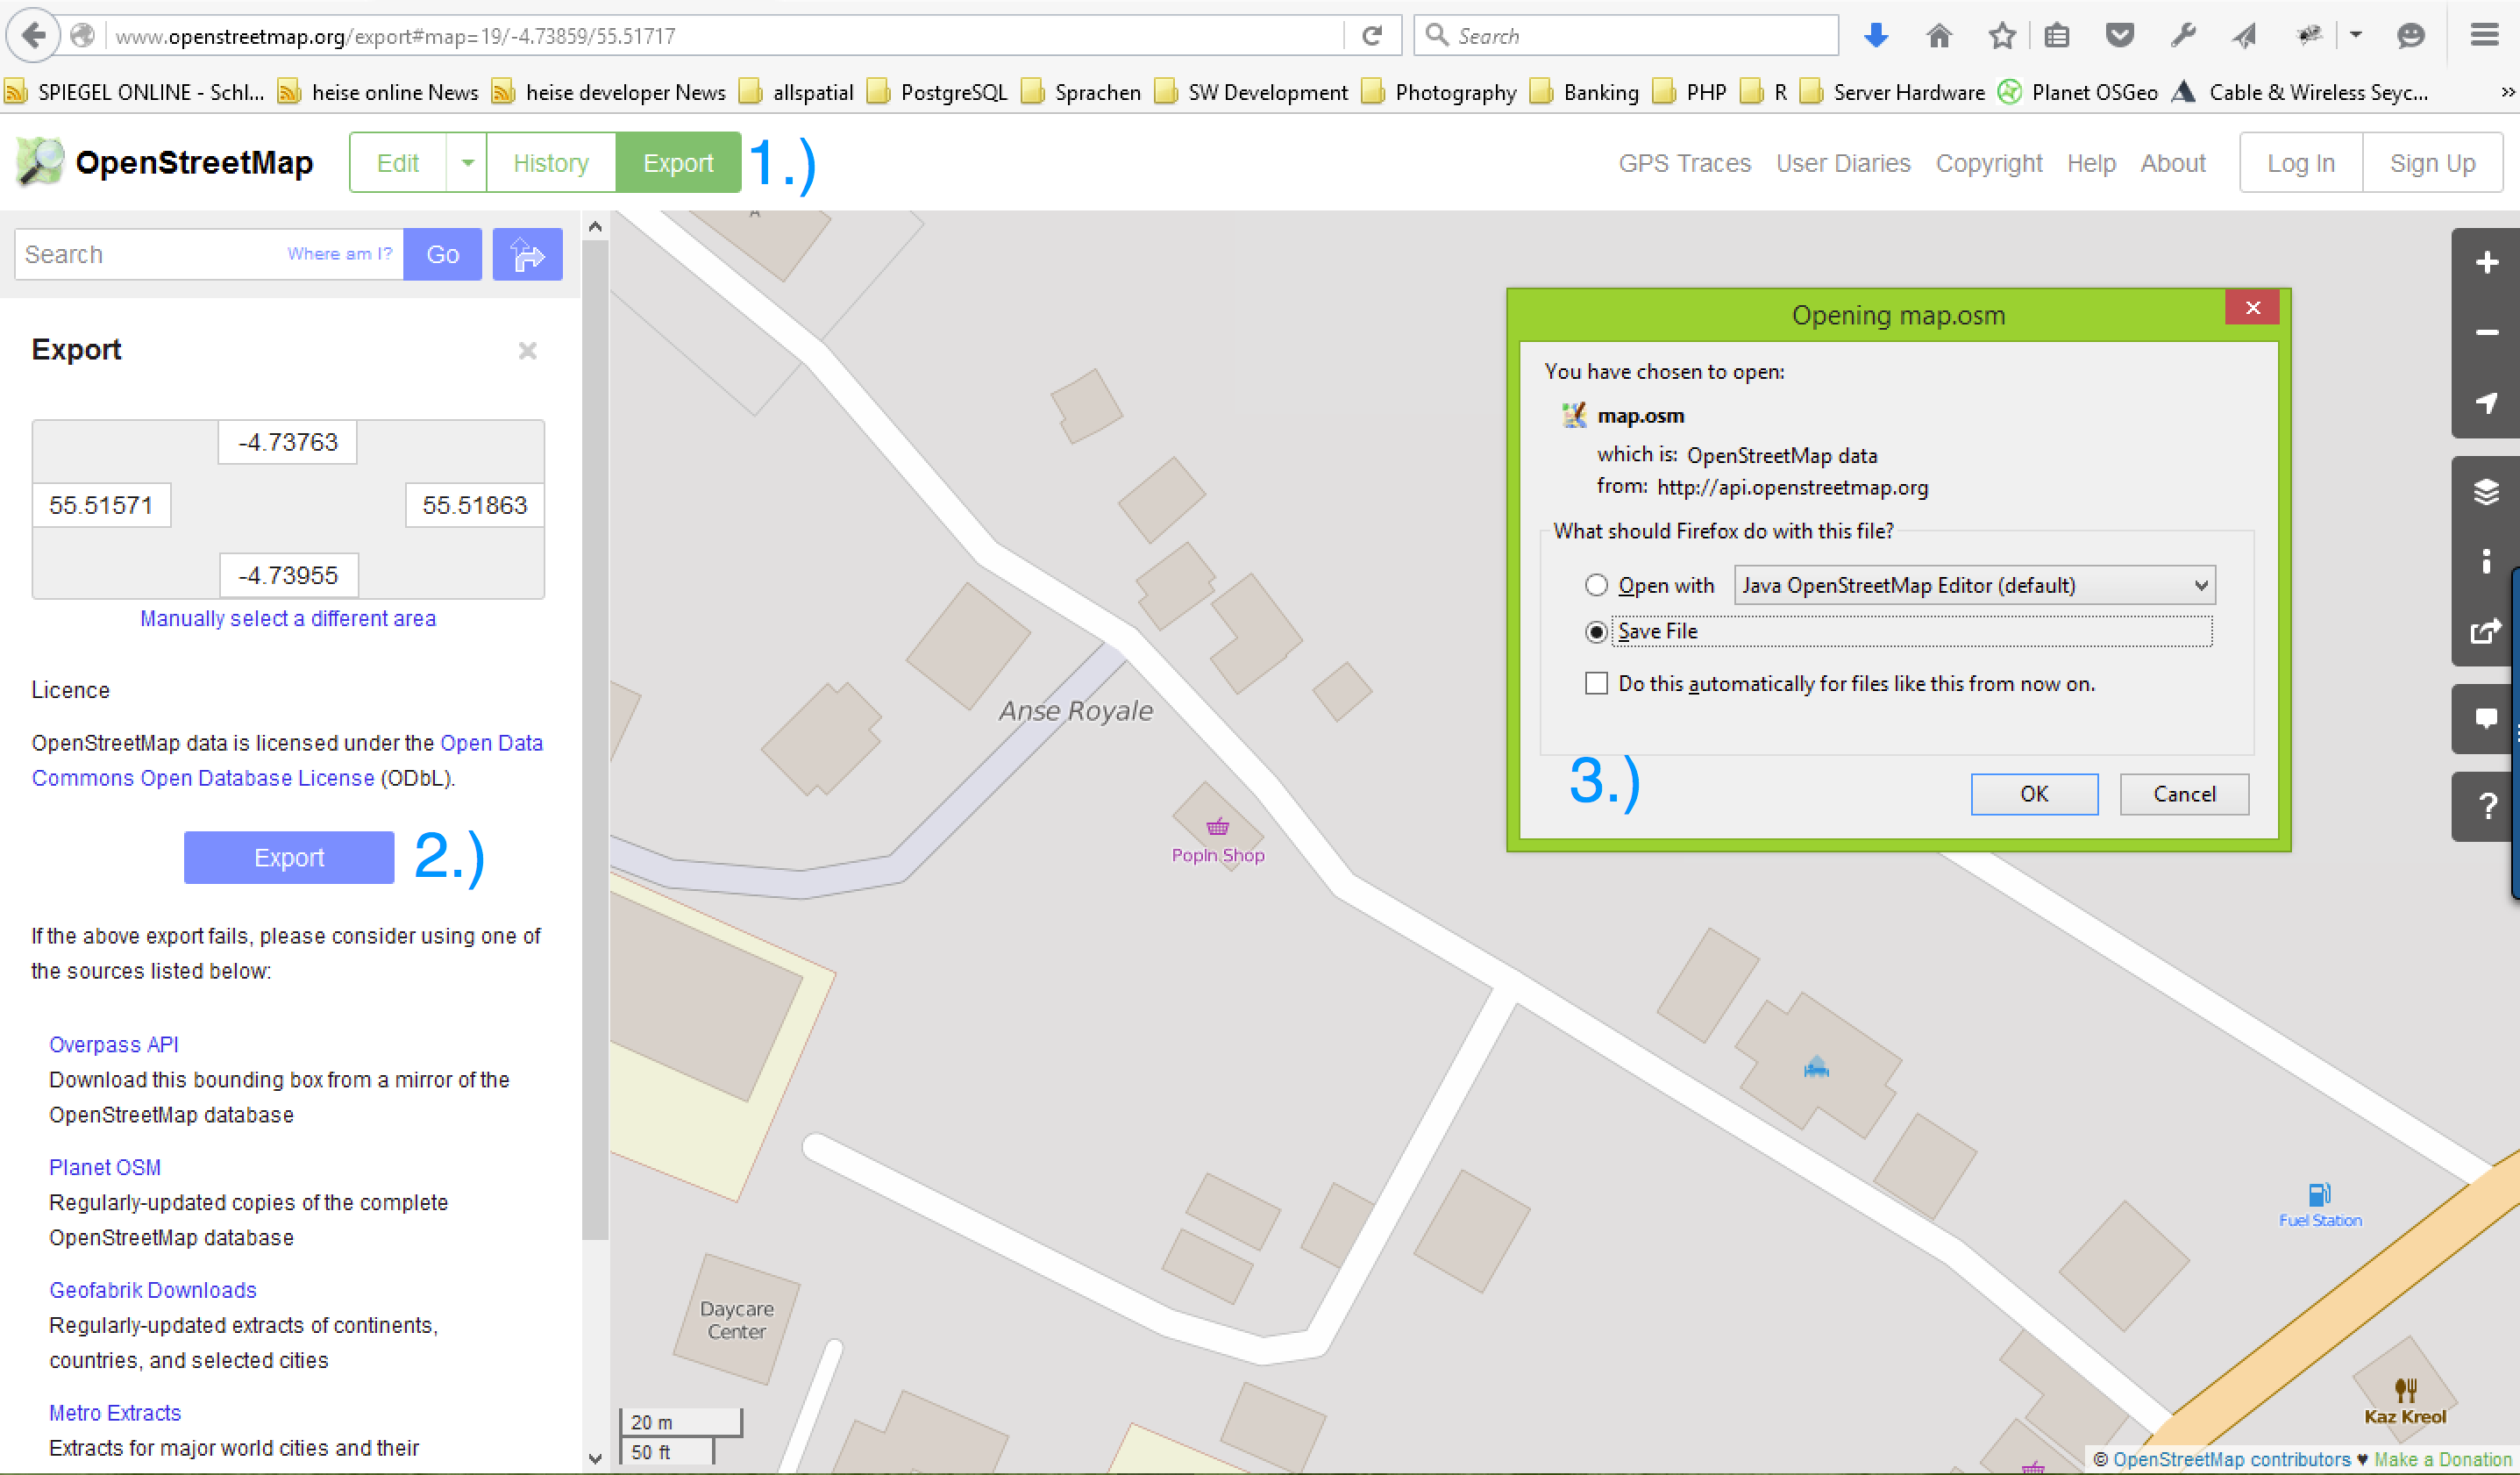
\includegraphics[width=12cm]{Images/import_1.png}
	\caption{Exporting OSM data from the OSM website}\label{fig:import_1}
\end{figure}

Launch QGIS and select \textit{Import Topology from XML...} from the \textit{Vector:OpenStreetMap} menu. Select the *.osm file you downloaded in the previous step.
Leave any other setting as provided by QGIS (Figure \ref{fig:import_2}).

 \begin{figure}[H]
 	\centering
 	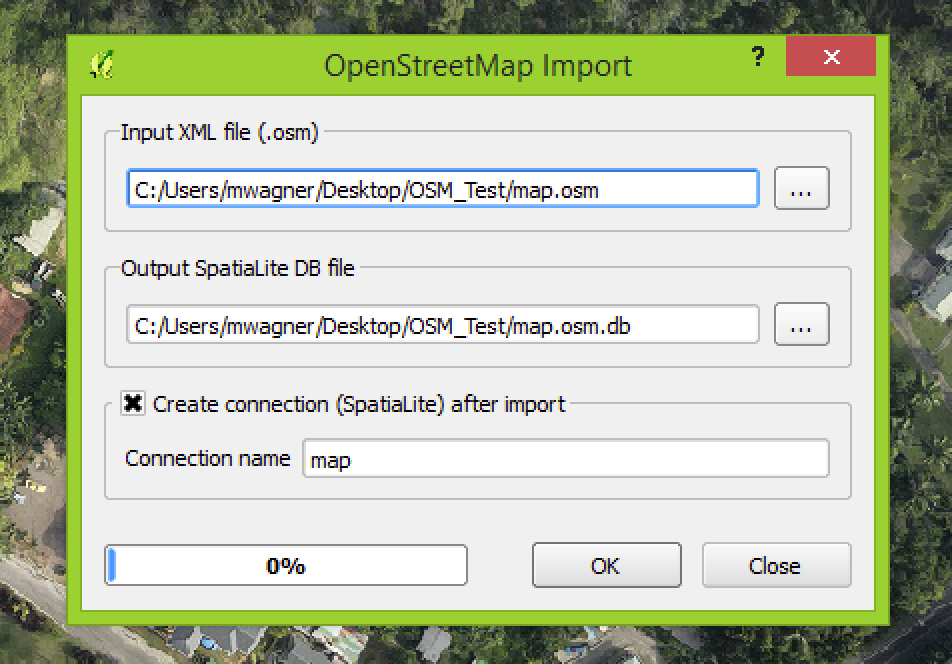
\includegraphics[width=8cm]{Images/import_2.png}
 	\caption{Importing OSM data into a SpatialLite database}\label{fig:import_2}
 \end{figure}
 
Select \textit{Export Topology to SpatialLite...} from the \textit{Vector:OpenStreetMap} menu. Select the SpatialLite database you created in the previous step and select the geometry type to export. Click the \textit{Load from DB} button to load all tags that are assigned to the selected geometry type (nodes, open ways and closed ways). Click \textit{Select All} to select all tags for the export and click the OK button. This will add a new layer to QGIS' Table of Content / legend (Figure \ref{fig:import_3}). Repeat this for the remaining geometry types.

 \begin{figure}[H]
 	\centering
 	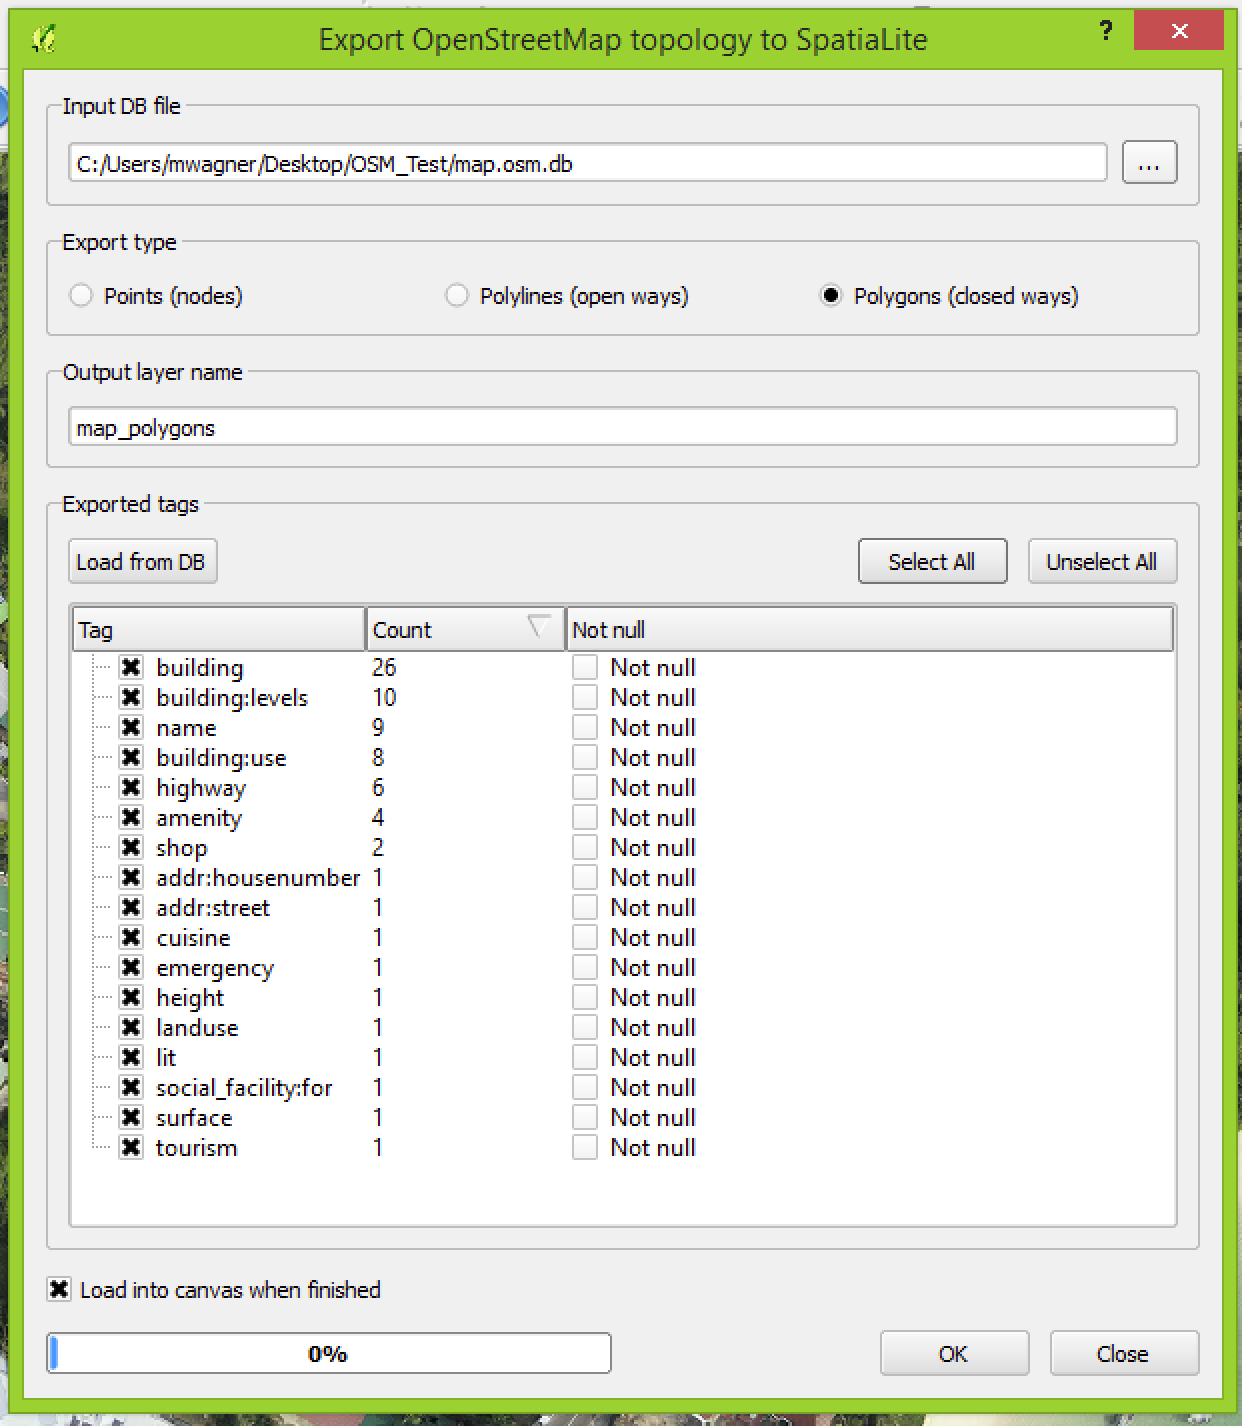
\includegraphics[width=8cm]{Images/import_3.png}
 	\caption{Exporting OSM data to a SpatialLite layer}\label{fig:import_3}
 \end{figure}
 
 As a result you should find three new layers in the legend (points, lines, polygons) that have all the originally assigned OSM tags as their attribute values. You can now filter and extract features based on these attribute values. To show only buildings from the polygon layer for example you could set a filter condition \textit{"building" IS NOT NULL} (Figure \ref{fig:import_4}).
 
 \begin{figure}[H]
 	\centering
 	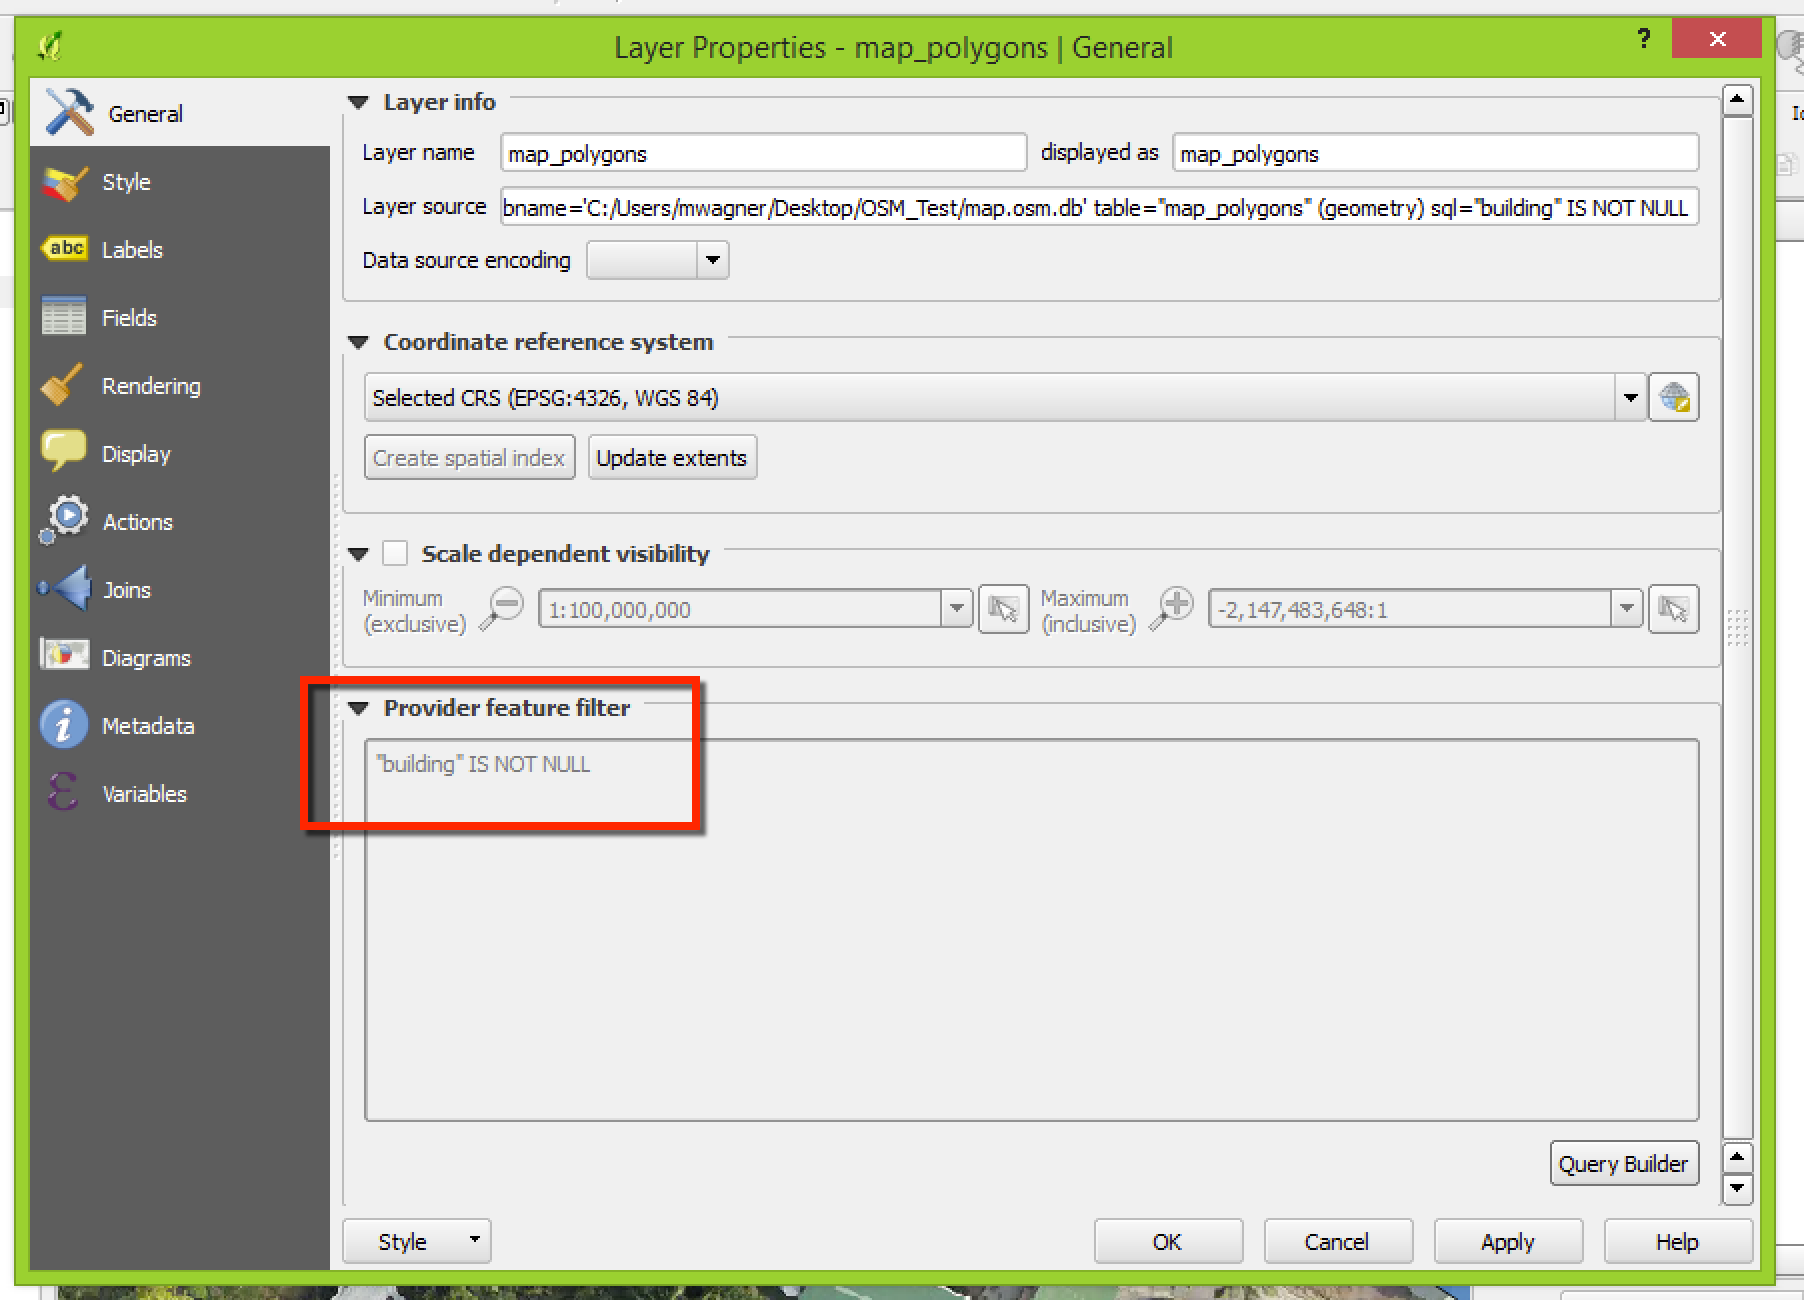
\includegraphics[width=8cm]{Images/import_4.png}
 	\caption{Setting a filter condition for a vector layer}\label{fig:import_4}
 \end{figure}
 
Those buildings still missing from your own \textit{building} layer you could then copy from the new layer into your own layer. To do this select the new layer in the legend and then select the buildings to be copied (Figure \ref{fig:import_5}). Press Ctrl+C to copy the buildings.

\begin{figure}[H]
	\centering
	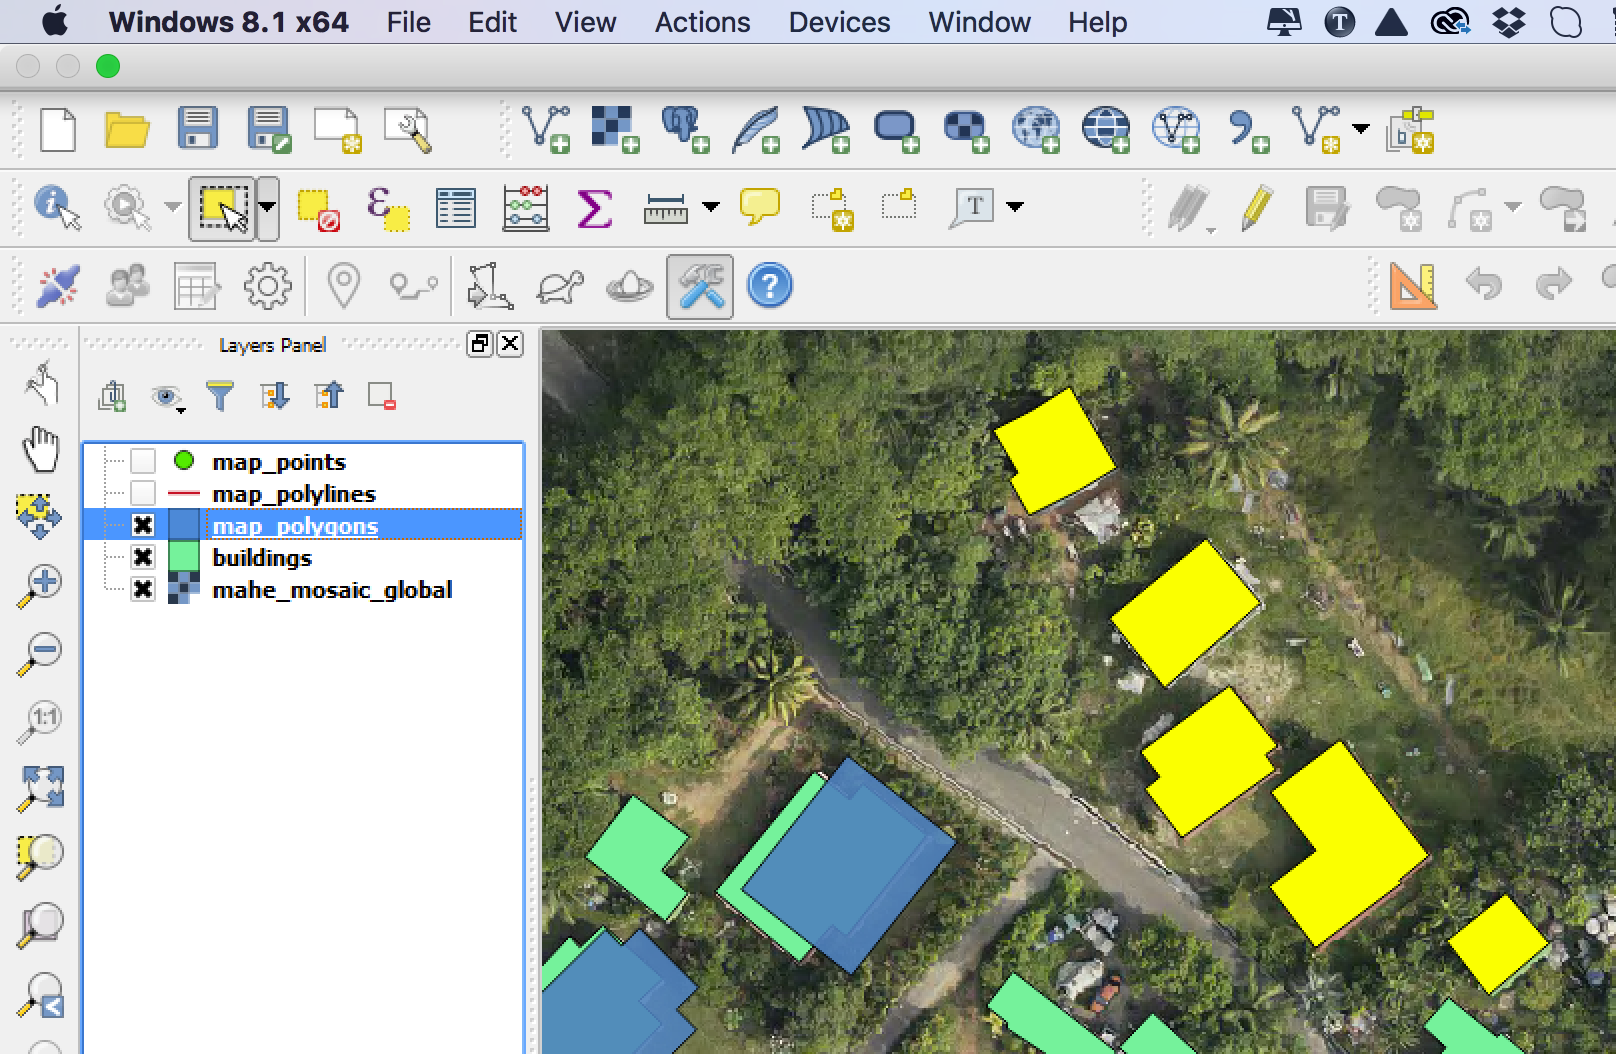
\includegraphics[width=12cm]{Images/import_5.png}
	\caption{Select buildings to be copied}\label{fig:import_5}
\end{figure}

Toggle the editing mode for your own \textit{building} layer (Figure \ref{fig:import_6}) and paste the new buildings into it by pressing Ctrl+V.

\begin{figure}[H]
	\centering
	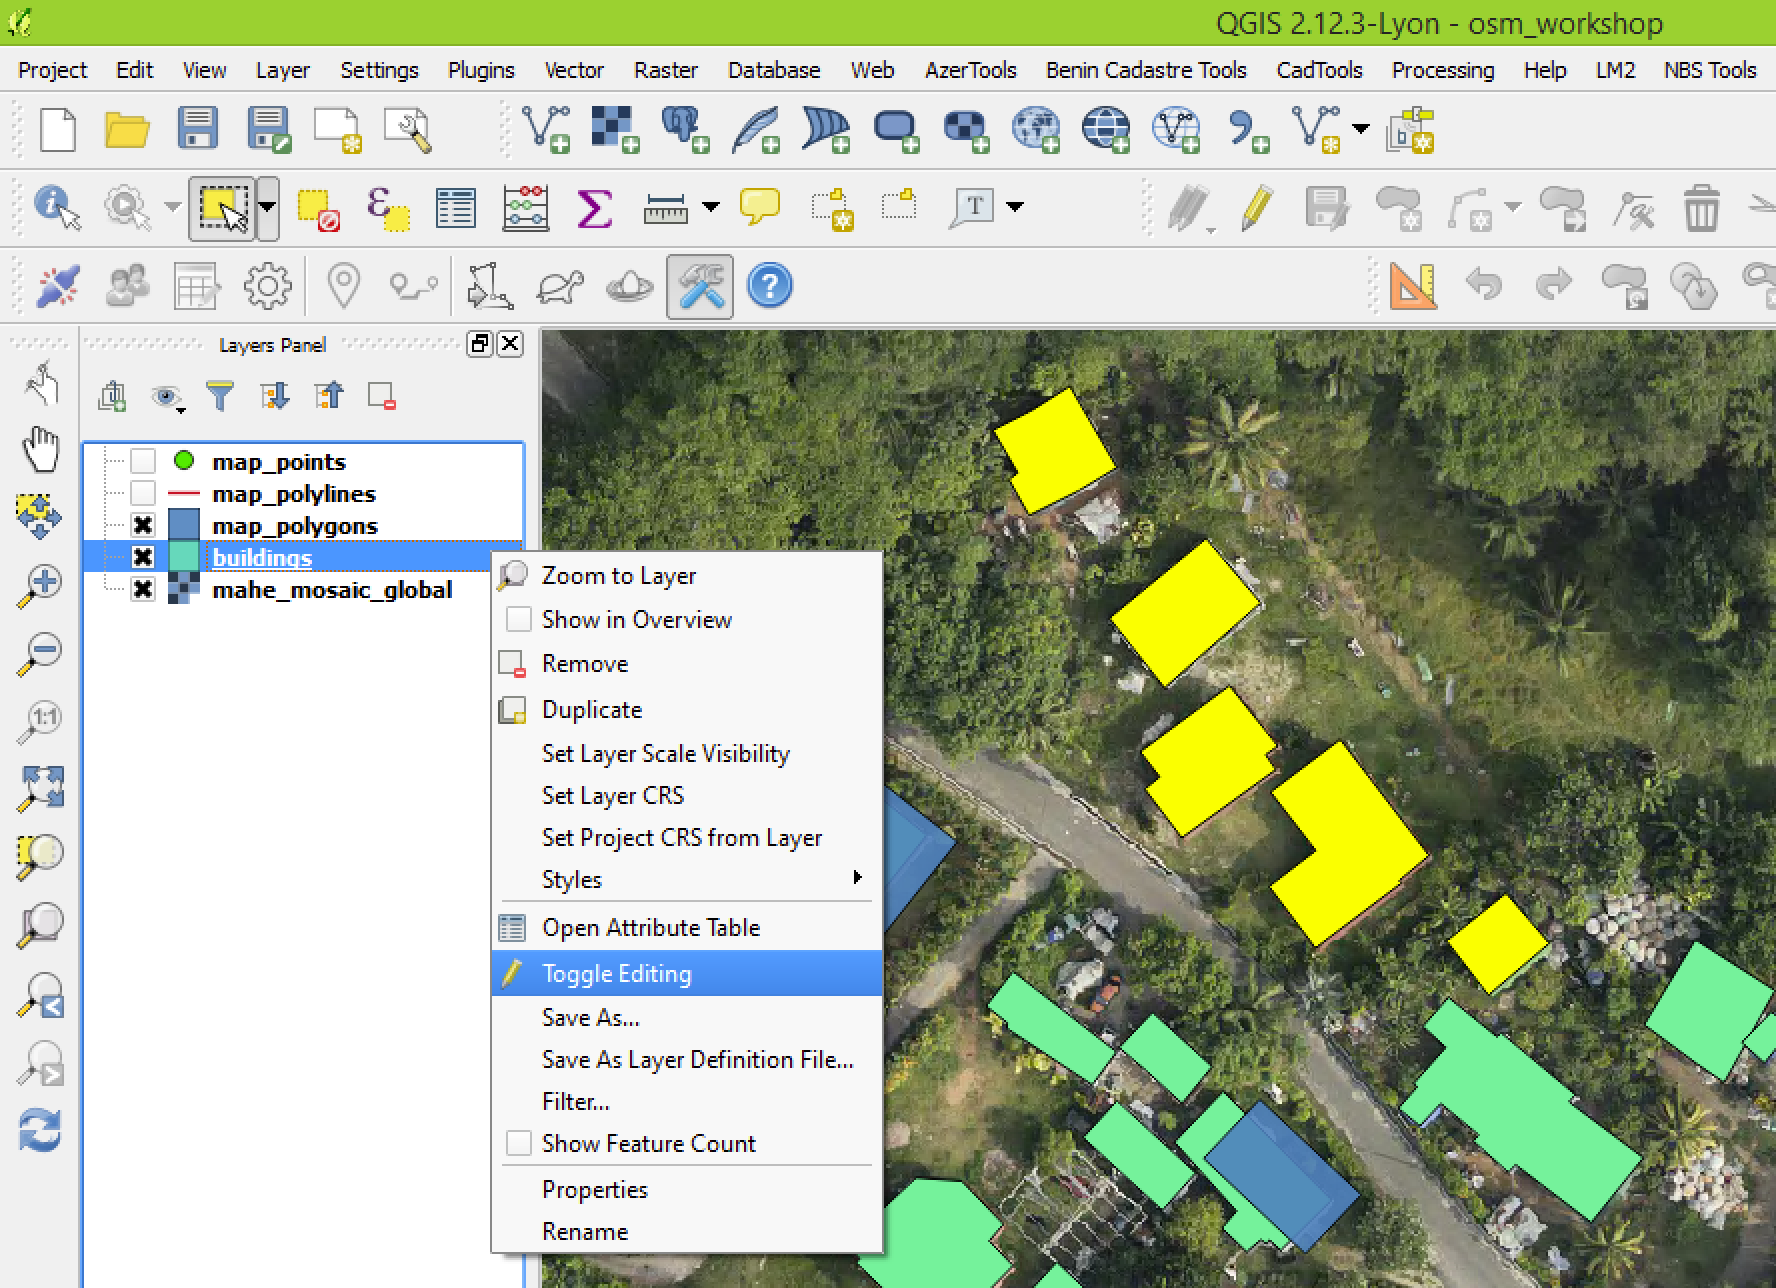
\includegraphics[width=12cm]{Images/import_6.png}
	\caption{Toggle editing mode}\label{fig:import_6}
\end{figure}

Save the edits by toggling edit mode again and the new buildings should appear in your own \textit{building} layer.

\end{document}
